% ============================================================================
% Accessibility
% ============================================================================
\DocumentMetadata{
  lang = en-US, 
  pdfstandard = ua-2, 
  tagging = on, 
  tagging-setup = {math/setup=mathml-SE}
}

% ============================================================================
% Document Properties - used on title slide and PDF metadata fields
% ============================================================================
\def\PresTitle{Angular Measurement}  % Required - top line of title slide
\def\PresSubtitle{Gauges and Measurement}         % Optional - second line
\def\PresAuthor{Brad Peirson}               % Required - below dividing line
\def\PresInstitute{College of Information Technology and Engineering}       % Optional
\def\PresDate{}                             % Optional
\def\PresKeywords{}                         % Optional - used for hyperref

% Presentation Formatting
% ============================================================================
% ============================================================================
% Class Declaration
% ============================================================================
\documentclass[
        mode = handout,     % Projector = one bullet at a time, Handout = all
        font-size=14pt,     % Only accepts 9, 10, 12, 14, 17, 20
        pdfusetitle         % Pulls \title property from document
    ]
    {ltx-talk}              % ltx-talk class

% ============================================================================
% Custom Colors
% ============================================================================
\usepackage[table]{xcolor}
% Colors from the Baker College Style Guide
%\definecolor{BakerADARed}{RGB}{231, 0, 46}   % #e7002e Official ADA red-doesn't pass WCAG AAA for small text
\definecolor{BakerADARed}{RGB}{181, 0, 36}    % #b50024 Adjusted ADA red-passes WCAG AAA for small text
\definecolor{HoneyYellow}{RGB}{255, 196, 0}   % #ffc400
\definecolor{UpNorthGreen}{RGB}{114, 191, 68} % #72bf44
\definecolor{LakeBlue}{RGB}{134, 183, 227}    % #86b7e3
\definecolor{BakerADI}{RGB}{58, 98, 170}
\definecolor{BakerCIM}{RGB}{217, 35, 47}
\definecolor{BakerBlack}{RGB}{31, 34, 40}     % #1f2228
\definecolor{BakerWhite}{RGB}{255, 255, 255}
\definecolor{BakerRed}{RGB}{239, 0, 48}
\definecolor{Abbey}{RGB}{80, 82, 88}
\definecolor{RollingStone}{RGB}{121, 124, 126}
\definecolor{HitGray}{RGB}{165, 169, 172}
\definecolor{Iron1}{RGB}{201, 206, 209}
\definecolor{Iron}{RGB}{222, 225, 226}
\definecolor{BlackHaze1}{RGB}{237, 240, 240}
\definecolor{BlackHaze}{RGB}{245, 247, 247}

% ============================================================================
% Document Data
% ============================================================================
\title{\PresTitle}
\author{\PresAuthor}
\institute{\PresInstitute}
\date{\PresDate}

%Set up the hyperlink colors
\hypersetup{colorlinks,
    linkcolor=BakerBlack,
    urlcolor=BakerADARed,
    pdfauthor = {\PresAuthor},
    %pdftitle = {\PresentationTopic},   % Title is pulled directly
    pdfsubject = {\PresSubtitle},
    pdfkeywords = {\Keywords},
    pdfcreator = {LaTeX with hyperref package},
    pdfproducer = {LuaLaTeX}
    }

% Map your custom style guide colors to the progress bar aliases
\colorlet{pbcomplete}{BakerADARed}
\colorlet{pbincomplete}{Iron}

\usepackage[most]{tcolorbox}

% ============================================================================
% Footer Format
% ============================================================================
\EditInstance{footer}{std}{
  color         = Abbey,
  separator     = \hfill,
  element-order = {title, institute, framenumber},
  right-hspace  = 3mm,
  left-hspace   = 3mm,
}

% \DeclareInstance{footer}{empty}{
%   element-order = {}
% }

% ============================================================================
% Progress Bar Toggles & Helper Macros
% ============================================================================
\usepackage{xfp}        % Needed for floating point math
\newif\ifprogressbar    % Used to determine whether or not to show the bar
\progressbartrue        % Set the bar to true at the start

% Helper macro to automatically turn off the progress bar inside title/section frames
\newcommand{\makeblindframe}[1]{%
  \progressbarfalse
  #1%
  \progressbartrue
}

% ============================================================================
% Custom Page Formats
% ============================================================================
\let\oldmaketitle\maketitle         % Backup the original maketitle command
\let\oldsection\section             % Backup the original section command
\let\oldsubsection\subsection       % Backup the original subsection command

\makeatletter
\renewcommand{\maketitle}{%
\makeblindframe{%
  \disableglobalbackground
  \slidebackground{PresentationTitleGraphic_2048x1151}%
  \color{white}%
  %\UseInstance{footer}{wallpaper}
  \begin{frame}
    \vspace*{1in}%
      \begin{tcolorbox}[
          enhanced,
          colback=black,       
          colframe=black,      
          opacityfill=0.25,       
          arc=6pt,                
          boxrule=0pt,            
          left=20pt, right=20pt,  
          top=20pt, bottom=20pt,
          width=0.80\textwidth,   
          halign=left             
      ]
          \color{white}%
          % Title (Always visible)
          {\large\bfseries\sffamily \@title}\\[0.5em]%
          
          % Conditional Subtitle
          \ifx\PresSubtitle\empty
          \else
            {\normalsize\sffamily \PresSubtitle}\\[0.5em]%
          \fi
          
          % High-contrast divider line
          {\color{white!80}\rule{0.3\textwidth}{0.8pt}}\\[0.5em]%
          
          % Author (Always visible)
          {\small\sffamily \@author}\\%
          
          % Conditional Institute
          \ifx\PresInstitute\empty
          \else
            {\small\sffamily \PresInstitute}\\%
          \fi
          
          % Conditional Date
          \ifx\PresDate\empty
          \else
            {\small\sffamily \@date}\\%
          \fi
      \end{tcolorbox}%
      \vfill     
  \end{frame}%
  \enableglobalbackground{BG}%
  \color{black}%
  %\UseInstance{footer}{std}
}%
}
\makeatother

% Create a variable container to hold the current section title
\newcommand{\currentsectiontitle}{}

% Redefine \section to take 1 argument (the title)
\renewcommand{\section}[1]{%
\makeblindframe{%
  \renewcommand{\currentsectiontitle}{#1}%
  \disableglobalbackground
  \slidebackground{PresentationSectionBackground_2048x1151}%
  \begin{frame}
    \vfill
    %\vspace*{0.625in}%
    \begin{tcolorbox}[
        enhanced,
        colback=black,       
        colframe=black,      
        opacityfill=0.25,       
        arc=6pt,                
        boxrule=0pt,            
        left=20pt, right=20pt,  
        top=20pt, bottom=20pt,
        width=0.80\textwidth,   
        halign=left             
    ]
        \color{white}%
        {\large\bfseries\sffamily #1}\\[0.5em]%   
    \end{tcolorbox}%
    \vfill 
  \end{frame}%
  \oldsection{#1}%
  \enableglobalbackground{BG}%

  % This will be used for an auto TOC at every section
  % Right now ltx-talk TOC is still in development
  % Once it comes a little further along this can be used
  % \begin{frame}
  %       \frametitle{Section Overview}
  %       \tableofcontents[sections=\thesection]
  %   \end{frame}%
}%
}

% Redefine \subsection to take 1 argument
\renewcommand{\subsection}[1]{%
\makeblindframe{%
  \disableglobalbackground
  \slidebackground{PresentationSectionBackground_2048x1151}%
  \begin{frame}
    \vfill
    %\vspace*{0.25in}% 
    \begin{tcolorbox}[
        enhanced,
        colback=black,       
        colframe=black,      
        opacityfill=0.25,       
        arc=6pt,                
        boxrule=0pt,            
        left=20pt, right=20pt,  
        top=20pt, bottom=20pt,
        width=0.80\textwidth,   
        halign=left             
    ]
        \color{white}%
        {\large\bfseries\sffamily\currentsectiontitle}\\[0.5em]%
        {\normalsize\sffamily #1}%
    \end{tcolorbox}%
    \vfill 
  \end{frame}%
  \oldsubsection{#1}%
  \enableglobalbackground{BG}%
}%
}

%Set the fonts to use NeueHaas Grotesk
\setsansfont{NHAASGROTESKTXPRO-}[
    Path=../NeueHaasGroteskFiles/,
    Scale=1.0,
    Extension = .ttf,
    UprightFont=*55Rg,
    BoldFont=*75Bd,
    ItalicFont=*56It,
    BoldItalicFont=*76BdIt
    ]

% Force the document default family to Sans-Serif
\renewcommand{\familydefault}{\sfdefault}

\usepackage{mathtools} % Load BEFORE unicode math settings
\setmathfont{Fira Math}[Scale=MatchLowercase] 

% 1. Turn global background ON
\newcommand{\enableglobalbackground}[1]{%
  \AddToHook{shipout/background}[mybg]{%
    \put(0, -\paperheight){%
      \includegraphics[width=\paperwidth, height=\paperheight, artifact]{#1}%
    }%
  }%
}

% 2. Turn global background OFF
\newcommand{\disableglobalbackground}{%
  \RemoveFromHook{shipout/background}[mybg]%
}

\newcommand{\slidebackground}[1]{%
  \AddToHookNext{shipout/background}{%
    \put(0, -\paperheight){%
      \includegraphics[width=\paperwidth, height=\paperheight, artifact]{#1}%
    }%
  }%
}

% --- GLOBAL BULLET OVERRIDES ---
\renewcommand{\labelitemi}{\color{BakerBlack}\Large\textbullet}
\renewcommand{\labelitemii}{\color{BakerBlack}\large\textbullet}
\renewcommand{\labelenumi}{\color{BakerBlack}\bfseries\arabic{enumi}.}
\renewcommand{\labelenumii}{\color{BakerBlack}\bfseries\alph{enumii})}

\AddToHook{begindocument/before}{%
  \EditInstance{item}{description}{
    label-format = \normalfont\bfseries\color{BakerADARed}#1
  }%
}

\AddToHook{begindocument/before}{%
  \EditInstance{item}{basic}{
    label-format = \color{BakerADARed}#1
  }%
}

% Global override for ltx-talk slide titles
\EditInstance{frametitle}{header}{
    font = \rule{0pt}{1.5cm}\bfseries\Large,
}

\EditInstance{header}{std}{
    font = \bfseries\huge,
    color = BakerBlack,
}

\AddToHook{env/block/begin}{%
  \colorlet{structure}{BakerADARed}%
}

\pretocmd{\tableofcontents}{\begin{minipage}{\textwidth} \linespread{1.4}}{}{}
\apptocmd{\tableofcontents}{\end{minipage}}{}{}

%Biber not functional in ltx-talk as of 2026-05-29
%Package that allows the creation of bibliographies
\usepackage[
    backend=biber,
    style=authoryear,
    sorting=none,
    %entryhead=false
    ]{biblatex}

%Load the bibliography file
\addbibresource{../../reference.bib}

\defbibheading{bibslide}{References}

\newcolumntype{L}[1]{>{\raggedright\let\newline\\\arraybackslash\hspace{0pt}}m{#1}}
\newcolumntype{C}[1]{>{\centering\let\newline\\\arraybackslash\hspace{0pt}}m{#1}}
\newcolumntype{R}[1]{>{\raggedleft\let\newline\\\arraybackslash\hspace{0pt}}m{#1}}

%All of the graphics are in a seperate folder, this makes it so the folder doesn't have to be repeated every time
\graphicspath{
  {../assets/images}
  {../assets/diagrams}
  {../assets/plots}
}

\makeatletter
% New counter to hold the custom "max frames" for the progress bar
\newcommand{\pb@maxtotal}{1}

% Read the custom total from the .aux file if it exists
\AtBeginDocument{%
  \ifdefined\pb@storedtotal
    \let\pb@maxtotal\pb@storedtotal
  \else
    % Fallback to standard total if our custom hook hasn't run yet
    \edef\pb@maxtotal{\@totalframes}%
  \fi
}

% Custom Appendix command that caps the progress bar and turns it off
\newcommand{\talkappendix}{%
  % 1. Write the CURRENT frame number to the .aux file as the progress total
  \immediate\write\@auxout{\string\gdef\string\pb@storedtotal{\@framenumber}}%
  % 2. Turn off the progress bar for all subsequent appendix slides
  \progressbarfalse
}
\makeatother

% ============================================================================
% Progress Bar Logic 
% ============================================================================
\makeatletter               
\AddToHook{shipout/background}{%
  \ifprogressbar
    % Read ltx-talk's internal frame counter safely
    \edef\currentframe{\@framenumber}%
    \edef\totalframes{\pb@maxtotal}% Use our custom max total instead
    
    % Fallback checks: If the document hasn't fully compiled yet, default to 1
    \ifx\currentframe\empty\def\currentframe{1}\fi
    \ifx\totalframes\empty\def\totalframes{1}\fi
    
    % Draw the progress bar if we have a valid total frame count
    \ifnum\totalframes>1\relax
      % Compute fraction width: (current - 1) / (total - 1)
      \edef\pbfraction{\fpeval{(\currentframe - 1) / (\totalframes - 1)}}%
      
      % Guard rails to prevent the bar from overshooting 100% on a first compile
      \ifdim\pbfraction pt>1pt\def\pbfraction{1}\fi 
      
      \edef\completewidth{\fpeval{\pbfraction * \paperwidth}}%
      \edef\incompletewidth{\fpeval{\paperwidth - \completewidth}}%
      
      % Render full-width progress bar at the top edge
      \put(0cm, -0.1cm){%
        \color{pbcomplete}\rule{\completewidth pt}{2pt}%
        \color{pbincomplete}\rule{\incompletewidth pt}{2pt}%
      }%
    \fi
  \fi
}
\makeatother

% 1. Globally shrink all caption components right as the caption engine fires
\AddToHook{cmd/@makecaption/before}{\footnotesize}

% 2. Declare and assign a blank plug to the kernel's caption label socket
\NewSocketPlug{caption/label}{nolabel}{}
\AssignSocketPlug{caption/label}{nolabel}

\usepackage{adjustbox}

\usepackage{amssymb}
\usepackage{amsmath}
\usepackage{siunitx}

\usepackage{animate}

\usepackage{calc} % Optional, but helpful for layout

\usepackage{multirow}

\usepackage{textcomp}

\usepackage{booktabs}
\usepackage{tabularx}

\usepackage[americanvoltages]{circuitikz}
\usepackage{pgfplots}
\usepackage{pgf-pie}

\usetikzlibrary{
    intersections, 
    fillbetween,
    patterns,
    decorations.pathreplacing,
    decorations.pathmorphing,
    decorations.text,
    decorations.markings,
    arrows.meta,
    arrows,
    shapes,
    shapes.geometric,
    shadows,
    calligraphy,
    backgrounds,
    intersections,
    calc,
    math,
    positioning,
    svg.path,
    shadows,
    shadows.blur,
    spy,
    }

\pgfplotsset{compat=1.18}

\pgfdeclarelayer{ft}
\pgfdeclarelayer{bg}
\pgfsetlayers{bg, main, ft}

% Usage: \hexpic[]{height}{Alt text}{Attribution}{image path}
\newcommand{\hexpic}[5][]{%
  \begin{figure}
    \centering
    \begin{tikzpicture}[
      baseline=(hex.base),      
      every shadow/.style={
        shadow opacity=70
        }
      ]
      \node (hex) [
        draw=white, 
        minimum size=#2, 
        regular polygon, 
        regular polygon sides=6, 
        rotate=90,
        blur shadow
      ] {};
      \begin{scope}
        \clip (hex.corner 1) -- (hex.corner 2) -- (hex.corner 3) -- 
              (hex.corner 4) -- (hex.corner 5) -- (hex.corner 6) -- cycle;
        \node at (hex.center) [#1] {
          \includegraphics[height=#2, alt={#3}]{#5}
        };
      \end{scope}
    \end{tikzpicture}

    \vspace{0.5em}
    {\tiny #4\par}
  \end{figure}  
}

% Usage: \shadowpic[]{width}{Alt text}{Attribution}{image path}
\newcommand{\shadowpic}[5][]{%
  \begin{figure}
    \centering
    \begin{tikzpicture}
      [every shadow/.style={
        shadow opacity=70
        }
      ]
      \node (image) [
        inner sep=0,
        blur shadow
      ] {\includegraphics[width=#2, alt={#3}]{#5}};
    \end{tikzpicture}

    \vspace{0.5em}
    {\tiny #4\par}
  \end{figure}
}

\tikzset{middlearrow/.style={
        decoration={markings, 
        mark= at position 0.5 with {\arrow{#1}},
        },
        postaction={decorate}
    }
}

% Usage: \tikztodo[width]{height}{description/notes}
\newcommand{\tikztodo}[3][0.8\textwidth]{%
  \begin{center}
    \fbox{%
      \parbox[c][#2][c]{#1}{%
        \centering
        \textbf{\textcolor{red}{TODO: TikZ Diagram}}\\[0.5em]
        \small #3%
      }%
    }%
  \end{center}%
}

% Macro: \drawrails{<number_of_1cm_segments>}
\newcommand{\drawrails}[1]{
  % Calculate total depth: 1 cm per segment
  \pgfmathsetmacro{\railheight}{-1 * #1}
  
  % L1 Rail (x = 0)
  \draw[thick] (0, 0) -- (0, \railheight cm);
    
  % L2 Rail (x = 15)
  \draw[thick] (15, 0) -- (15, \railheight cm);
}

\newcommand{\ccwplus}{%
  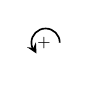
\begin{tikzpicture}[baseline=(char.base)]
    \node(char) at (0,0) {\(\scriptscriptstyle +\)};
    \draw[->, >=stealth, semithick] (0.2,0) arc (0:230:0.18cm);
  \end{tikzpicture}%
}

%====================================================================================
% Timer Ladder Symbol - Could be used for TON, TOF, RTO....
%====================================================================================
\tikzset{
    TON/.pic={

        \draw[
          BakerBlack
        ]
        (0,0)
        -- ++(0,0.375)
        -- ++(3.5,0)
        coordinate[pos=0.5](-TOP)
        -- ++(0,-1.75)
        coordinate[pos=3/14](-OUT)
        coordinate[pos=0.5](-EN1)
        coordinate[pos=0.875](-DN1)
        -- ++(-3.5,0)        
        -- (0,0)
        coordinate(-IN);

        \node[
          text=BakerBlack,
          font=\bfseries,
          anchor=east
        ](pre)
        at ($(-TOP)-(0,1.75em)$)
        {{\small PRE:}};

        \node[
          text=BakerBlack,
          font=\bfseries,
          anchor=east
        ](acc)
        at ($(pre.east)-(0,1em)$)
        {{\small ACC:}};

        \coordinate (-PRE) at (pre.east); % For the preset value
        \coordinate (-ACC) at (acc.east);

        \draw[
            BakerBlack
        ]
        (-EN1)
        -- ++(0.5,0)
        coordinate(-EN2)
        node[
            text=BakerBlack,
            anchor=west
        ]
        {{\small EN}};

        \draw[
            BakerBlack
        ]
        (-DN1)
        -- ++(0.5,0)
        coordinate(-DN2)
        node[
            text=BakerBlack,
            anchor=west
        ]
        {{\small DN}};

    }
}

%====================================================================================
% Oval ladder symbol, good for ONS, RES, etc.
%====================================================================================
\tikzset{
    ONS/.pic={

        \draw[
          BakerBlack
        ]
        (0,0)
        coordinate(-IN)
        -- ++(0.75,0)
        node[
          draw=BakerBlack, 
          text=BakerBlack, 
          font=\small, 
          minimum width=1.5cm, 
          minimum height=0.75cm, 
          anchor=west, 
          rounded corners=0.25cm
          ](ons){};
        
        \draw[BakerBlack] (ons.east) -- ++(0.75,0) coordinate(-OUT);

        \coordinate(-INS) at (ons.center);
        \coordinate(-VAR) at (ons.north); 
    }
}

%====================================================================================
% Source A, Source B, Dest box
%====================================================================================
\tikzset{
    SrcDest/.pic={
      
        \draw[
          BakerBlack
        ]
        (0,0)
        coordinate(-IN)
        -- ++(0,0.375)
        -- ++(5,0)
        coordinate[pos=0.5](-TOP)
        -- ++(0,-3.25)
        coordinate[pos=3/26](-OUT)
        -- ++(-5,0)
        -- (0,0)
        coordinate(l1);

        \node[
          text=BakerBlack,
          font=\bfseries,
          anchor=west
        ](srcA)
        at (l1)
        {{\small Src A:}};

        \node[
          text=BakerBlack,
          font=\bfseries,
          anchor=west
        ](srcB)
        at ($(l1)-(0,2em)$)
        {{\small Src B:}};

        \node[
          text=BakerBlack,
          font=\bfseries,
          anchor=west
        ](dest)
        at ($(srcB.west)-(0,2em)$)
        {{\small Dest:}};

        \coordinate(-SRCA) at (srcA.east);
        \coordinate(-AVAL) at ($(srcA.east)-(0,1em)$);
        \coordinate(-SRCB) at (srcB.east);
        \coordinate(-BVAL) at ($(srcB.east)-(0,1em)$);
        \coordinate(-DEST) at ($(-BVAL)-(0,1em)$);
        \coordinate(-DVAL) at ($(-DEST)-(0,1em)$);
    }
}

%====================================================================================
% Source A, Source B box
%====================================================================================
\tikzset{
    SrcAB/.pic={
      
        \draw[
          BakerBlack
        ]
        (0,0)
        coordinate(-IN)
        -- ++(0,0.375)
        -- ++(4,0)
        coordinate[pos=0.5](-TOP)
        -- ++(0,-2.25)
        coordinate[pos=1/6](-OUT)
        -- ++(-4,0)
        -- (0,0)
        coordinate(l1);

        \node[
          text=BakerBlack,
          font=\bfseries,
          anchor=west
        ](srcA)
        at (l1)
        {{\small Src A:}};

        \node[
          text=BakerBlack,
          font=\bfseries,
          anchor=west
        ](srcB)
        at ($(l1)-(0,2em)$)
        {{\small Src B:}};

        \coordinate(-SRCA) at (srcA.east);
        \coordinate(-AVAL) at ($(srcA.east)-(0,1em)$);
        \coordinate(-SRCB) at (srcB.east);
        \coordinate(-BVAL) at ($(srcB.east)-(0,1em)$);
    }
}

%====================================================================================
% LIMIT instruction
%====================================================================================
\tikzset{
    Limit/.pic={
      
        \draw[
          BakerBlack
        ]
        (0,0)
        coordinate(-IN)
        -- ++(0,0.375)
        -- ++(4,0)
        coordinate[pos=0.5](-TOP)
        -- ++(0,-3.25)
        coordinate[pos=3/26](-OUT)
        -- ++(-4,0)
        -- (0,0)
        coordinate(l1);

        \node[
          text=BakerBlack,
          font=\bfseries,
          anchor=west
        ](srcA)
        at (l1)
        {{\small Low:}};

        \node[
          text=BakerBlack,
          font=\bfseries,
          anchor=west
        ](srcB)
        at ($(l1)-(0,2em)$)
        {{\small Test:}};

        \node[
          text=BakerBlack,
          font=\bfseries,
          anchor=west
        ](dest)
        at ($(srcB.west)-(0,2em)$)
        {{\small High:}};

        \coordinate(-LO) at (srcA.east);
        \coordinate(-LOV) at ($(srcA.east)-(0,1em)$);
        \coordinate(-TEST) at (srcB.east);
        \coordinate(-TESTV) at ($(srcB.east)-(0,1em)$);
        \coordinate(-HI) at ($(-TESTV)-(0,1em)$);
        \coordinate(-HIV) at ($(-HI)-(0,1em)$);
    }
}

%====================================================================================
% Source Destination box
%====================================================================================
\tikzset{
    SrcSingle/.pic={
      
        \draw[
          BakerBlack
        ]
        (0,0)
        coordinate(-IN)
        -- ++(0,0.375)
        -- ++(6,0)
        coordinate[pos=0.5](-TOP)
        -- ++(0,-2.25)
        coordinate[pos=1/6](-OUT)
        -- ++(-6,0)
        -- (0,0)
        coordinate(l1);

        \node[
          text=BakerBlack,
          font=\bfseries,
          anchor=west
        ](srcA)
        at (l1)
        {{\small Source:}};

        \node[
          text=BakerBlack,
          font=\bfseries,
          anchor=east
        ](srcB)
        at ($(srcA.east)-(0,2em)$)
        {{\small Dest:}};

        \coordinate(-SRC) at (srcA.east);
        \coordinate(-SRCV) at ($(srcA.east)-(0,1em)$);
        \coordinate(-DEST) at (srcB.east);
        \coordinate(-DESTV) at ($(srcB.east)-(0,1em)$);
    }
}

%====================================================================================
% Compute Box
%====================================================================================
\tikzset{
    CPT/.pic={
      
        \draw[
          BakerBlack
        ]
        (0,0)
        coordinate(-IN)
        -- ++(0,0.375)
        -- ++(8.5,0)
        coordinate[pos=0.5](-TOP)
        -- ++(0,-1.75)
        coordinate[pos=3/14](-OUT)
        -- ++(-8.5,0)
        -- (0,0)
        coordinate(l1);

        \node[
          text=BakerBlack,
          font=\bfseries,
          anchor=west
        ](srcA)
        at (l1)
        {{\small Source:}};

        \node[
          text=BakerBlack,
          font=\bfseries,
          anchor=east
        ](srcB)
        at ($(srcA.east)-(0,2em)$)
        {{\small Exp:}};

        \coordinate(-DEST) at (srcA.east);
        \coordinate(-DESTV) at ($(srcA.east)-(0,1em)$);
        \coordinate(-EXP) at (srcB.east);
        \coordinate(-EXPV) at ($(srcB.east)-(0,1em)$);
    }
}

% ============================================================================
% Document Content
% ============================================================================
\begin{document}

\maketitle              % Redefined in the preamble to generate a full frame

\begin{frame}
    \frametitle{Agenda}
    \begingroup
        % Tighten the spacing between paragraphs/TOC lines
        \setlength{\parskip}{0.3em} 
        
        % Optionally tighten the line spacing within an entry
        %\baselineskip=1.2em 
        
        \setcounter{tocdepth}{1} % Show only sections
    \tableofcontents
    \setcounter{tocdepth}{2} % Reset back to default so subsections are tracked
    \endgroup
\end{frame}

\section{Introduction}

\begin{frame}
	\frametitle{Angular Measurement}

    \begin{columns}
        \begin{column}{0.48\linewidth}
            \shadowpic[]{\linewidth}{An antique brass sextant displayed flat against a pale gray fabric background, with a small rectangular label numbered 6 near the bottom right corner.}{\textbf{Attribution:} \href{https://commons.wikimedia.org/wiki/File:Sextante_(1805)._Museo_Naval_de_Madrid.jpg}{Jerónimo Roure Pérez}, \href{http://creativecommons.org/licenses/by-sa/4.0/}{CC BY-SA 4.0}, via Wikimedia Commons}{Sextante_(1805)._Museo_Naval_de_Madrid}
        \end{column}
        \begin{column}{0.48\linewidth}
            \shadowpic[]{0.5\linewidth}{A land surveying pole supported by a black and neon green bipod stands over a metal survey marker in a field of tall dry grass, with a yellow handheld data collector mounted to the pole and a red metal fence post tied with pink flagging tape standing just to the left under a blue sky with distant mountains and white clouds.}{\textbf{Attribution:} \href{https://commons.wikimedia.org/wiki/File:Land_Survey_(14000483127).jpg}{Bureau of Land Management Oregon and Washington}, Public domain, via Wikimedia Commons}{Land_Survey_(14000483127)}
        \end{column}
    \end{columns}
\end{frame}

\begin{frame}
	\frametitle{The Protractor}

    \begin{columns}
        \begin{column}{0.48\linewidth}
            \begin{itemize}[<+- | alert@+>]
                \item Many angular measurement techniques available in mechatronics
                \item Protractor is the most basic
            \end{itemize}
        \end{column}
        \begin{column}{0.48\linewidth}
            \shadowpic[]{\linewidth}{A metal universal bevel protractor with a circular graduated dial, locking knobs, and a long beveled straightedge resting on a solid blue background.}{\textbf{Attribution:} \href{https://commons.wikimedia.org/wiki/File:Universal_bevel_protractor_against_blue_background.jpg}{Connie Posites}, \href{https://creativecommons.org/licenses/by-sa/2.0}{CC BY-SA 2.0}, via Wikimedia Commons}{Universal_bevel_protractor_against_blue_background}
        \end{column}
    \end{columns}
\end{frame}            

\begin{frame}
	\frametitle{Digital Protractors}

    \begin{columns}
        \begin{column}{0.48\linewidth}
            \begin{itemize}[<+- | alert@+>]
                \item Like other measurement methods, digital has taken over
                \item Remember: batteries die
                \item Still important to know the fundamentals
            \end{itemize}
        \end{column}
        \begin{column}{0.48\linewidth}
            \shadowpic[]{\linewidth}{A stainless steel digital protractor ruler with two hinged arms marked in metric and imperial graduations, featuring a black digital display unit on the right showing an angle reading of 24.7 degrees against a plain white background.}{\textbf{Attribution:} \href{https://commons.wikimedia.org/wiki/File:Digital_protractor_powerfix.jpg}{wdwd}, \href{https://creativecommons.org/licenses/by-sa/4.0}{CC BY-SA 4.0}, via Wikimedia Commons}{Digital_protractor_powerfix}
        \end{column}
    \end{columns}
\end{frame}

\section{Trigonometry}

\subsection{Basic Geometry}

\begin{frame}
	\frametitle{The Line}

    \begin{columns}
        \begin{column}{0.48\linewidth}
            \begin{itemize}[<+- | alert@+>]
                \item A \emph{line} is one-dimensional
                    \begin{itemize}
                        \item Only has a length
                        \item Its width is infinitely small
                    \end{itemize}                
            \end{itemize}
        \end{column}
        \begin{column}{0.48\linewidth}
            \centering
            \begin{tikzpicture}[alt={A straight, red line drawn angled slightly up and to the right.}]
                \draw[BakerADARed, ultra thick, drop shadow] (0,0) -- (6,4);
            \end{tikzpicture}
        \end{column}
    \end{columns}
\end{frame}

\begin{frame}
	\frametitle{The Plane}

    \begin{columns}
        \begin{column}{0.48\linewidth}
            \begin{itemize}[<+- | alert@+>]
                \item A \emph{plane} is two dimensional
                    \begin{itemize}
                        \item Length and width
                        \item Thickness is infinitely small
                    \end{itemize}
                \item A plane is a line swept in a single direction
            \end{itemize}
        \end{column}
        \begin{column}{0.48\linewidth}
            \centering
            \resizebox{\linewidth}{!}{
                \begin{circuitikz}[
    american, 
    >={Latex[length=5mm, width=2mm]},
    alt={A parallelogram filled with semi-transparent light red, featuring thick solid blue diagonal sides on the left and right, dashed red horizontal sides on the top and bottom, and a thick black horizontal arrow pointing to the right in the center.}
    ]

    \begin{pgfonlayer}{ft}
    
        \draw[
            LakeBlue,
            ultra thick
        ]
        (0,0)
        -- ++(4,4)
        coordinate(ul);

        \draw[
            BakerADARed,
            dashed
        ]
        (ul)
        -- ++(6,0)
        coordinate(ur);

        \draw[
            LakeBlue,
            ultra thick
        ]
        (ur)
        -- ++(-4,-4)
        coordinate(lr);

        \draw[
            BakerADARed,
            dashed
        ]
        (lr)
        -- (0,0);

    \end{pgfonlayer}

    \begin{pgfonlayer}{bg}

        \fill[
            fill=BakerADARed!50,
            fill opacity=0.5
        ]
        (0,0)
        -- (ul)
        -- (ur)
        -- (lr)
        -- cycle;
    
    \end{pgfonlayer}

    \begin{pgfonlayer}{main}
        \draw[
            BakerBlack,
            ultra thick,
            ->
        ]
        (4,2)
        -- (6,2);
    \end{pgfonlayer}

\end{circuitikz}
            }
        \end{column}
    \end{columns}
\end{frame}

\begin{frame}
	\frametitle{Plane Flatness}

    \begin{columns}
        \begin{column}{0.48\linewidth}
            \begin{itemize}[<+- | alert@+>]
                \item A plane is created from a line
                \item Lines are perfectly straight
                \item Planes are perfectly flat
            \end{itemize}
        \end{column}
        \begin{column}{0.48\linewidth}
            \centering
            \resizebox{\linewidth}{!}{
                \begin{circuitikz}[
    american, 
    >={Latex[length=5mm, width=2mm]},
    alt={A parallelogram filled with semi-transparent light red, featuring thick solid blue diagonal sides on the left and right, dashed red horizontal sides on the top and bottom, and a thick black horizontal arrow pointing to the right in the center.}
    ]

    \begin{pgfonlayer}{ft}
    
        \draw[
            LakeBlue,
            ultra thick
        ]
        (0,0)
        -- ++(4,4)
        coordinate(ul);

        \draw[
            BakerADARed,
            dashed
        ]
        (ul)
        -- ++(6,0)
        coordinate(ur);

        \draw[
            LakeBlue,
            ultra thick
        ]
        (ur)
        -- ++(-4,-4)
        coordinate(lr);

        \draw[
            BakerADARed,
            dashed
        ]
        (lr)
        -- (0,0);

    \end{pgfonlayer}

    \begin{pgfonlayer}{bg}

        \fill[
            fill=BakerADARed!50,
            fill opacity=0.5
        ]
        (0,0)
        -- (ul)
        -- (ur)
        -- (lr)
        -- cycle;
    
    \end{pgfonlayer}

    \begin{pgfonlayer}{main}
        \draw[
            BakerBlack,
            ultra thick,
            ->
        ]
        (4,2)
        -- (6,2);
    \end{pgfonlayer}

\end{circuitikz}
            }
        \end{column}
    \end{columns}
\end{frame}

\begin{frame}
	\frametitle{The Angle}

    \begin{columns}
        \begin{column}{0.48\linewidth}
            \begin{itemize}[<+- | alert@+>]
                \item Picture one end of a line pinned in place
                \item As it rotates around that point it sweeps in an arc
                \item An \emph{angle} is the amount of rotation the line makes around the fixed point
            \end{itemize}
        \end{column}
        \begin{column}{0.48\linewidth}
            \centering
            \resizebox{\linewidth}{!}{
                \begin{circuitikz}[
    american, 
    >={Latex[length=5mm, width=2mm]},
    alt={A circular sector filled with semi-transparent light red, bounded by a thick black horizontal bottom radius, a thick blue upper radius angled at sixty degrees, and a thick dashed red curved arc with an arrow pointing counterclockwise from the bottom edge to the top edge.}
    ]

    \begin{pgfonlayer}{ft}
    
        % \node[
        %     draw=BakerBlack,
        %     fill=BakerBlack,
        %     circle,
        %     inner sep=0,
        %     minimum size=0.25cm
        % ]
        % at (0,0)
        % {};

    \end{pgfonlayer}

    \begin{pgfonlayer}{main}

        \draw[
            BakerBlack,
            ultra thick
        ]
        (0,0)
        -- ++(6,0)
        coordinate(right);

        \draw[
            BakerADARed,
            ultra thick,
            dashed,
            ->
        ]
        (right)
        arc[start angle=0, end angle=60, radius=6cm];

        \draw[
            LakeBlue,
            ultra thick
        ]
        (0,0)
        -- (60:6cm);
    
    \end{pgfonlayer}

    \begin{pgfonlayer}{bg}
        \fill[
            fill=BakerADARed!50,
            fill opacity=0.5
        ]
        (0,0)
        -- (6,0)
        arc[start angle=0, end angle=60, radius=6cm]
        -- cycle;
    \end{pgfonlayer}

\end{circuitikz}
            }
        \end{column}
    \end{columns}
\end{frame}

\begin{frame}
	\frametitle{The Circle}

    \begin{columns}
        \begin{column}{0.48\linewidth}
            \begin{itemize}[<+- | alert@+>]
                \item A \emph{circle} is the path traced by the moving end of the line when it makes a complete rotation
                \item Every time the line sweeps it creates an angle
                \item Circles are made up of infinite angles
            \end{itemize} 
        \end{column}
        \begin{column}{0.48\linewidth}
            \centering
            \resizebox{\linewidth}{!}{
                \begin{circuitikz}[
    american, 
    >={Latex[length=5mm, width=2mm]},
    alt={A full circle filled with semi-transparent light red, featuring a thick black horizontal radius extending to the right edge, four closely spaced blue radii angled slightly above the horizontal at ten, twelve, fourteen, and sixteen degrees, and a thick dashed red perimeter with an arrow pointing counterclockwise around the circumference back to the right edge.}
    ]

    \begin{pgfonlayer}{ft}
    
        % \node[
        %     draw=BakerBlack,
        %     fill=BakerBlack,
        %     circle,
        %     inner sep=0,
        %     minimum size=0.25cm
        % ]
        % at (0,0)
        % {};

    \end{pgfonlayer}

    \begin{pgfonlayer}{main}

        \draw[
            BakerBlack,
            ultra thick
        ]
        (0,0)
        -- ++(3,0)
        coordinate(right);

        \draw[
            LakeBlue,
            thick
        ]
        (0,0)
        -- (10:3cm);

        \draw[
            LakeBlue,
            thick
        ]
        (0,0)
        -- (12:3cm);

        \draw[
            LakeBlue,
            thick
        ]
        (0,0)
        -- (14:3cm);

        \draw[
            LakeBlue,
            thick
        ]
        (0,0)
        -- (16:3cm);

        \draw[
            BakerADARed,
            ultra thick,
            dashed,
            ->
        ]
        (right)
        arc[start angle=0, end angle=360, radius=3cm];
    
    \end{pgfonlayer}

    \begin{pgfonlayer}{bg}
        \node[
            fill=BakerADARed!50,
            fill opacity=0.5,
            circle,
            minimum size=6cm
        ]
        at (0,0)
        {};

    \end{pgfonlayer}

\end{circuitikz}
            }
        \end{column}
    \end{columns}
\end{frame}

\subsection{Degree Measurement}

\begin{frame}
	\frametitle{Degrees}

    \begin{columns}
        \begin{column}{0.48\linewidth}
            \begin{itemize}[<+- | alert@+>]
                \item Angles exist, we need to measure them
                \item Angular measurement is as old as human history
            \end{itemize} 
        \end{column}
        \begin{column}{0.48\linewidth}
            \shadowpic[]{0.75\linewidth}{A circular translucent orange plastic protractor with a horizontal crossbar across its center and black degree markings from zero to three hundred sixty around the perimeter against a plain white background.}{\textbf{Attribution:} \href{https://commons.wikimedia.org/wiki/File:Protractor_katomierz.jpg}{Radomil}, \href{http://creativecommons.org/licenses/by-sa/3.0/}{CC BY-SA 3.0}, via Wikimedia Commons}{Protractor_katomierz}
        \end{column}
    \end{columns}
\end{frame}

\begin{frame}
	\frametitle{Degrees}

    \begin{itemize}[<+- | alert@+>]
        \item Ancient Sumerians, Babylonians, Mesopotamians used a base-60 number system
            \begin{itemize}
                \item Based around their calculation of the length of a year
            \end{itemize}
        \item Egyptians inherited base-60 numbers--used it to divide a circle into 360 equal divisions
        \item Like most imperial units, handy mental calculation
            \begin{itemize}
                \item 360 equally divides by 2, 3, 4, 5, 6, 8, 9, 10, 12\dots
            \end{itemize}
        \item Each of the 360 divisions is one \emph{degree} (\textdegree{})
    \end{itemize}
\end{frame}

\begin{frame}
	\frametitle{Minutes and Seconds}

    \begin{columns}[t]
        \begin{column}{0.48\linewidth}
            \begin{itemize}[<+- | alert@+>]
                \item A circle has an infinite number of angles in it
                \item An angle can be smaller than 1\textdegree{}
                \item Each degree is further divided by 60
                \item Not included on measurement devices--would be too small to read
            \end{itemize} 
        \end{column}
        \begin{column}{0.48\linewidth}
            \begin{itemize}[<+- | alert@+>]
                \item 1 degree divided by 60 equals 1 minute
                    \begin{itemize}
                        \item $\ang{1} / 60 = \ang{;1}$
                    \end{itemize}
                \item 1 minute divided by 60 equals 1 second
                    \begin{itemize}
                        \item $\ang{;1} / 60 = \ang{;;1}$
                    \end{itemize}
            \end{itemize} 
        \end{column}
    \end{columns}
\end{frame}

\begin{frame}
	\frametitle{Ex 1: Degrees, Minutes, Seconds}

    Consider an angle that takes up one fourteenth of a circle:

    \begin{align*}
        \ang{360} / 14 &= \ang{25.7143}\\
        \ang{0.7143} \times 60 &= \ang{;42.858}\\
        \ang{0.858} \times 60 &= \ang{;;51.48}\\
        \ang{360} / 14 &= \ang{25;42;51}
    \end{align*}
\end{frame}

\begin{frame}
	\frametitle{Ex 2: Degrees, Minutes, Seconds (1 of 2)}

    Convert $\ang{129.37}$ to degrees, minutes, and seconds:

    % \begin{align*}
    %     \ang{0.37} \times 60 &= \ang{;22.2}\\
    %     \ang{0.2} \times 60 &= \ang{;;12}\\
    %     \ang{129.37} &= \ang{129;22;12}
    % \end{align*}
    
\end{frame}

\begin{frame}
	\frametitle{Ex 2: Degrees, Minutes, Seconds (2 of 2)}

    Convert $\ang{129.37}$ to degrees, minutes, and seconds:

    \begin{align*}
        \ang{0.37} \times 60 &= \ang{;22.2}\\
        \ang{0.2} \times 60 &= \ang{;;12}\\
        \ang{129.37} &= \ang{129;22;12}
    \end{align*}
    
\end{frame}

\subsection{Radian Measurement}

\begin{frame}
	\frametitle{The Radian}

    \begin{columns}
        \begin{column}{0.48\linewidth}
            \begin{itemize}[<+- | alert@+>]
                \item A \emph{radian} is a an angular unit that arose in the 1400s
                \item The angle created when the arc traced by the line is equal to the length of the line
            \end{itemize}
        \end{column}
        \begin{column}{0.48\linewidth}
            \centering
            \resizebox{\linewidth}{!}{
                \begin{circuitikz}[
    american, 
    >={Latex[length=5mm, width=2mm]},
    alt={A circular sector filled with semi-transparent light red, bounded by a thick black horizontal bottom radius labeled l, a thick blue upper radius labeled l angled at one radian, and a thick dashed red curved outer arc labeled l with an arrow pointing counterclockwise from the bottom edge to the top edge, with a thin green inner arc between the two radii labeled 1 radian.}
    ]

    \pgfmathsetmacro{\myangle}{deg(pi)}

    \begin{pgfonlayer}{ft}
    
        % \node[
        %     draw=BakerBlack,
        %     fill=BakerBlack,
        %     circle,
        %     inner sep=0,
        %     minimum size=0.25cm
        % ]
        % at (0,0)
        % {};

    \end{pgfonlayer}

    \begin{pgfonlayer}{main}

        \draw[
            BakerBlack,
            ultra thick
        ]
        (0,0)
        -- (6,0)
        node[
            text=BakerBlack,
            midway,
            below
        ]{$l$};

        \draw[
            LakeBlue,
            ultra thick
        ]
        (0,0)
        -- (1r:6cm)
        node[
            text=BakerBlack,
            midway,
            anchor=south east
        ]{$l$};

        \draw[
            BakerADARed,
            ultra thick,
            dashed,
            ->
        ]
        (6,0)
        arc[start angle=0, end angle=1r, radius=6cm]
        node[
            text=BakerBlack,
            midway,
            right
        ]{$l$};

        \draw[
            UpNorthGreen,
            thick
        ]
        (2,0)
        arc[start angle=0, end angle=1r, radius=2cm]
        node[
            text=BakerBlack,
            midway,
            right
        ]{$\qty{1}{\radian}$};

    \end{pgfonlayer}
    
    \begin{pgfonlayer}{bg}

        \fill[
            fill=BakerADARed!50,
            fill opacity=0.5
        ]
        (0,0)
        -- (6,0)
        arc[start angle=0, end angle=1r, radius=6cm]
        -- cycle;

    \end{pgfonlayer}
\end{circuitikz}
            }
        \end{column}
    \end{columns}
\end{frame}

\begin{frame}
	\frametitle{Radian History}

    \begin{columns}
        \begin{column}{0.48\linewidth}
            \begin{itemize}[<+- | alert@+>]
                \item First adopted by Leonhard Euler in 1765
                \item First mention in print in 1873
                \item Adopted as a \emph{supplementary} unit in the SI system in 1960
                    \begin{itemize}
                        \item Supplementary units are dimensionless in SI
                    \end{itemize}
            \end{itemize}
        \end{column}
        \begin{column}{0.48\linewidth}
            \shadowpic[]{0.625\linewidth}{A painted bust portrait of Leonhard Euler looking slightly to the left, wearing a draped light gray cap, a white ruffled cravat, and a blue coat with wide dark stripes against a dark background.}{\textbf{Attribution:} \href{https://commons.wikimedia.org/wiki/File:Leonhard_Euler_-_edit1.jpg}{Jakob Emanuel Handmann}, Public domain, via Wikimedia Commons}{Leonhard_Euler_-_Jakob_Emanuel_Handmann_(Kunstmuseum_Basel)}
        \end{column}
    \end{columns}
\end{frame}

\begin{frame}
	\frametitle{Radian Definition}

    \begin{columns}
        \begin{column}{0.48\linewidth}
            \begin{itemize}[<+- | alert@+>]
                \item Radian is based on the length of the arc drawn by the line
                \item One radian is the angle that occurs when the length of the arc is equal to the length of the line
            \end{itemize}
        \end{column}
        \begin{column}{0.48\linewidth}
            \centering
            \resizebox{\linewidth}{!}{
                \begin{circuitikz}[
    american, 
    >={Latex[length=5mm, width=2mm]},
    alt={A circular sector filled with semi-transparent light red, bounded by a thick black horizontal bottom radius labeled l, a thick blue upper radius labeled l angled at one radian, and a thick dashed red curved outer arc labeled l with an arrow pointing counterclockwise from the bottom edge to the top edge, with a thin green inner arc between the two radii labeled 1 radian.}
    ]

    \pgfmathsetmacro{\myangle}{deg(pi)}

    \begin{pgfonlayer}{ft}
    
        % \node[
        %     draw=BakerBlack,
        %     fill=BakerBlack,
        %     circle,
        %     inner sep=0,
        %     minimum size=0.25cm
        % ]
        % at (0,0)
        % {};

    \end{pgfonlayer}

    \begin{pgfonlayer}{main}

        \draw[
            BakerBlack,
            ultra thick
        ]
        (0,0)
        -- (6,0)
        node[
            text=BakerBlack,
            midway,
            below
        ]{$l$};

        \draw[
            LakeBlue,
            ultra thick
        ]
        (0,0)
        -- (1r:6cm)
        node[
            text=BakerBlack,
            midway,
            anchor=south east
        ]{$l$};

        \draw[
            BakerADARed,
            ultra thick,
            dashed,
            ->
        ]
        (6,0)
        arc[start angle=0, end angle=1r, radius=6cm]
        node[
            text=BakerBlack,
            midway,
            right
        ]{$l$};

        \draw[
            UpNorthGreen,
            thick
        ]
        (2,0)
        arc[start angle=0, end angle=1r, radius=2cm]
        node[
            text=BakerBlack,
            midway,
            right
        ]{$\qty{1}{\radian}$};

    \end{pgfonlayer}
    
    \begin{pgfonlayer}{bg}

        \fill[
            fill=BakerADARed!50,
            fill opacity=0.5
        ]
        (0,0)
        -- (6,0)
        arc[start angle=0, end angle=1r, radius=6cm]
        -- cycle;

    \end{pgfonlayer}
\end{circuitikz}
            }
        \end{column}
    \end{columns}
\end{frame}

\begin{frame}
	\frametitle{Radians Around a Circle (1 of 4)}

    \begin{columns}
        \begin{column}{0.48\linewidth}
            \centering
            \resizebox{\linewidth}{!}{
                \begin{circuitikz}[
    american, 
    >={Latex[length=5mm, width=2mm]},
    alt={}
    ]

    \pgfmathsetmacro{\myangle}{deg(pi)}

    \begin{pgfonlayer}{ft}
    
        % \node[
        %     draw=BakerBlack,
        %     fill=BakerBlack,
        %     circle,
        %     inner sep=0,
        %     minimum size=0.25cm
        % ]
        % at (0,0)
        % {};

    \end{pgfonlayer}

    \begin{pgfonlayer}{main}

        \draw[
            BakerBlack,
            ultra thick
        ]
        (0,0)
        -- (6,0)
        node[
            text=BakerBlack,
            midway,
            below
        ]{$l$};

        \draw[
            UpNorthGreen,
            ultra thick
        ]
        (0,0)
        -- (1r:6cm)
        node[
            text=BakerBlack,
            midway,
            anchor=south east
        ]{$l$};

        \draw[
            LakeBlue,
            ultra thick
        ]
        (0,0)
        -- (2r:6cm)
        node[
            text=BakerBlack,
            midway,
            anchor=north east
        ]{$l$};

        \draw[
            BakerADARed,
            ultra thick,
            dashed,
            ->
        ]
        (1r:6cm)
        arc[start angle=1r, end angle=2r, radius=6cm]
        node[
            text=BakerBlack,
            midway,
            above
        ]{$l$};

        \draw[
            UpNorthGreen,
            thick
        ]
        (2,0)
        arc[start angle=0, end angle=1r, radius=2cm]
        node[
            text=BakerBlack,
            midway,
            right
        ]{$\qty{1}{\radian}$};

        \draw[
            UpNorthGreen,
            thick
        ]
        (1r:2cm)
        arc[start angle=1r, end angle=2r, radius=2cm]
        node[
            text=BakerBlack,
            midway,
            above
        ]{$\qty{1}{\radian}$};

    \end{pgfonlayer}
    
    \begin{pgfonlayer}{bg}

        \fill[
            fill=BakerADARed!50,
            fill opacity=0.5
        ]
        (0,0)
        -- (6,0)
        arc[start angle=0, end angle=2r, radius=6cm]
        -- cycle;

    \end{pgfonlayer}
\end{circuitikz}
            }
        \end{column}
        \begin{column}{0.48\linewidth}
            \centering
            \resizebox{\linewidth}{!}{
                \begin{circuitikz}[
    american, 
    >={Latex[length=5mm, width=2mm]},
    alt={}
    ]

    \pgfmathsetmacro{\myangle}{deg(pi)}

    \begin{pgfonlayer}{ft}
    
        % \node[
        %     draw=BakerBlack,
        %     fill=BakerBlack,
        %     circle,
        %     inner sep=0,
        %     minimum size=0.25cm
        % ]
        % at (0,0)
        % {};

    \end{pgfonlayer}

    \begin{pgfonlayer}{main}

        \draw[
            BakerBlack,
            ultra thick
        ]
        (0,0)
        -- (6,0)
        node[
            text=BakerBlack,
            midway,
            below
        ]{$l$};

        \draw[
            UpNorthGreen,
            ultra thick
        ]
        (0,0)
        -- (1r:6cm)
        node[
            text=BakerBlack,
            midway,
            anchor=south east
        ]{$l$};

        \draw[
            UpNorthGreen,
            ultra thick
        ]
        (0,0)
        -- (2r:6cm)
        node[
            text=BakerBlack,
            midway,
            anchor=north east
        ]{$l$};

        \draw[
            LakeBlue,
            ultra thick
        ]
        (0,0)
        -- (3r:6cm)
        node[
            text=BakerBlack,
            midway,
            anchor=south west
        ]{$l$};

        \draw[
            BakerADARed,
            ultra thick,
            dashed,
            ->
        ]
        (2r:6cm)
        arc[start angle=2r, end angle=3r, radius=6cm]
        node[
            text=BakerBlack,
            midway,
            anchor=south east
        ]{$l$};

        \draw[
            UpNorthGreen,
            thick
        ]
        (2,0)
        arc[start angle=0, end angle=1r, radius=2cm]
        node[
            text=BakerBlack,
            midway,
            right
        ]{$\qty{1}{\radian}$};

        \draw[
            UpNorthGreen,
            thick
        ]
        (1r:2cm)
        arc[start angle=1r, end angle=2r, radius=2cm]
        node[
            text=BakerBlack,
            midway,
            above
        ]{$\qty{1}{\radian}$};

        \draw[
            UpNorthGreen,
            thick
        ]
        (2r:2cm)
        arc[start angle=2r, end angle=3r, radius=2cm]
        node[
            text=BakerBlack,
            midway,
            anchor=south east
        ]{$\qty{1}{\radian}$};

    \end{pgfonlayer}
    
    \begin{pgfonlayer}{bg}

        \fill[
            fill=BakerADARed!50,
            fill opacity=0.5
        ]
        (0,0)
        -- (6,0)
        arc[start angle=0, end angle=3r, radius=6cm]
        -- cycle;

    \end{pgfonlayer}
\end{circuitikz}
            }
        \end{column}
    \end{columns}
\end{frame}

\begin{frame}
	\frametitle{Radians Around a Circle (2 of 4)}

    \centering
    \resizebox{0.5\linewidth}{!}{
        \begin{circuitikz}[
    american, 
    >={Latex[length=5mm, width=2mm]},
    alt={}
    ]

    \pgfmathsetmacro{\myangle}{deg(pi)}

    \begin{pgfonlayer}{ft}
    
        % \node[
        %     draw=BakerBlack,
        %     fill=BakerBlack,
        %     circle,
        %     inner sep=0,
        %     minimum size=0.25cm
        % ]
        % at (0,0)
        % {};

    \end{pgfonlayer}

    \begin{pgfonlayer}{main}

        \draw[
            BakerBlack,
            ultra thick
        ]
        (0,0)
        -- (6,0)
        node[
            text=BakerBlack,
            midway,
            below
        ]{$l$};

        \draw[
            UpNorthGreen,
            ultra thick
        ]
        (0,0)
        -- (1r:6cm)
        node[
            text=BakerBlack,
            midway,
            anchor=south east
        ]{$l$};

        \draw[
            UpNorthGreen,
            ultra thick
        ]
        (0,0)
        -- (2r:6cm)
        node[
            text=BakerBlack,
            midway,
            anchor=north east
        ]{$l$};

        \draw[
            LakeBlue,
            ultra thick
        ]
        (0,0)
        -- (3r:6cm)
        node[
            text=BakerBlack,
            midway,
            anchor=south west
        ]{$l$};

        \draw[
            BakerADARed,
            ultra thick,
            dashed,
            ->
        ]
        (2r:6cm)
        arc[start angle=2r, end angle=3r, radius=6cm]
        node[
            text=BakerBlack,
            midway,
            anchor=south east
        ]{$l$};

        \draw[
            UpNorthGreen,
            thick
        ]
        (2,0)
        arc[start angle=0, end angle=1r, radius=2cm]
        node[
            text=BakerBlack,
            midway,
            right
        ]{$\qty{1}{\radian}$};

        \draw[
            UpNorthGreen,
            thick
        ]
        (1r:2cm)
        arc[start angle=1r, end angle=2r, radius=2cm]
        node[
            text=BakerBlack,
            midway,
            above
        ]{$\qty{1}{\radian}$};

        \draw[
            UpNorthGreen,
            thick
        ]
        (2r:2cm)
        arc[start angle=2r, end angle=3r, radius=2cm]
        node[
            text=BakerBlack,
            midway,
            anchor=south east
        ]{$\qty{1}{\radian}$};

        %============================================================
        % 180 degree line
        %============================================================
        \draw[
            BakerBlack,
            ultra thick,
            dashed
        ]
        (0,0)
        -- (-6,0);

        \draw[
            HoneyYellow,
            ultra thick
        ]
        (-2,0)
        arc[start angle=180, end angle=3r, radius=2cm]
        coordinate[midway](angCenter);

        \draw[
            BakerBlack,
            thick,
            dashed
        ]
        (2,0)
        arc[start angle=360, end angle=180, radius=2cm]
        node[
            text=BakerBlack,
            midway,
            below
        ]{$\ang{180}$};

        \draw[
            UpNorthGreen,
            thick,
            <-
        ]
        (angCenter)
        to[out=180, in=0]
        ++(-2,-1)
        node[
            text=BakerBlack,
            anchor=east
        ]{?};

    \end{pgfonlayer}
    
    \begin{pgfonlayer}{bg}

        \fill[
            fill=BakerADARed!50,
            fill opacity=0.5
        ]
        (0,0)
        -- (6,0)
        arc[start angle=0, end angle=3r, radius=6cm]
        -- cycle;

    \end{pgfonlayer}
\end{circuitikz}
    }

    \vspace{0.5em}
    {\footnotesize $\qty{3}{\radian}$ leaves us short of half a circle ($\ang{180}$)--care to guess \emph{how short?}\par}
\end{frame}

\begin{frame}
	\frametitle{Radians Around a Circle (3 of 4)}

    \centering
    \resizebox{0.5\linewidth}{!}{
        \begin{circuitikz}[
    american, 
    >={Latex[length=5mm, width=2mm]},
    alt={A circular sector filled with semi-transparent light red representing three radians, divided into three equal one-radian sectors by a thick black horizontal bottom radius, two thick green interior radii, and a thick blue upper radius slightly above the negative horizontal axis, with all four radii labeled l. A thick dashed red outer arc with an arrow points counterclockwise from the second green radius to the blue radius and is labeled l, while three thin green inner arcs each span one radian and are labeled 1 radian. A thick dashed black horizontal radius extends to the left to show the 180-degree line, with a thin dashed black lower semicircle arc labeled 180 degrees and a thick yellow arc filling the remaining gap between three radians and 180 degrees, pointed to by a green arrow labeled 0.141593... radians.}
    ]

    \pgfmathsetmacro{\myangle}{deg(pi)}

    \begin{pgfonlayer}{ft}
    
        % \node[
        %     draw=BakerBlack,
        %     fill=BakerBlack,
        %     circle,
        %     inner sep=0,
        %     minimum size=0.25cm
        % ]
        % at (0,0)
        % {};

    \end{pgfonlayer}

    \begin{pgfonlayer}{main}

        \draw[
            BakerBlack,
            ultra thick
        ]
        (0,0)
        -- (6,0)
        node[
            text=BakerBlack,
            midway,
            below
        ]{$l$};

        \draw[
            UpNorthGreen,
            ultra thick
        ]
        (0,0)
        -- (1r:6cm)
        node[
            text=BakerBlack,
            midway,
            anchor=south east
        ]{$l$};

        \draw[
            UpNorthGreen,
            ultra thick
        ]
        (0,0)
        -- (2r:6cm)
        node[
            text=BakerBlack,
            midway,
            anchor=north east
        ]{$l$};

        \draw[
            LakeBlue,
            ultra thick
        ]
        (0,0)
        -- (3r:6cm)
        node[
            text=BakerBlack,
            midway,
            anchor=south west
        ]{$l$};

        \draw[
            BakerADARed,
            ultra thick,
            dashed,
            ->
        ]
        (2r:6cm)
        arc[start angle=2r, end angle=3r, radius=6cm]
        node[
            text=BakerBlack,
            midway,
            anchor=south east
        ]{$l$};

        \draw[
            UpNorthGreen,
            thick
        ]
        (2,0)
        arc[start angle=0, end angle=1r, radius=2cm]
        node[
            text=BakerBlack,
            midway,
            right
        ]{$\qty{1}{\radian}$};

        \draw[
            UpNorthGreen,
            thick
        ]
        (1r:2cm)
        arc[start angle=1r, end angle=2r, radius=2cm]
        node[
            text=BakerBlack,
            midway,
            above
        ]{$\qty{1}{\radian}$};

        \draw[
            UpNorthGreen,
            thick
        ]
        (2r:2cm)
        arc[start angle=2r, end angle=3r, radius=2cm]
        node[
            text=BakerBlack,
            midway,
            anchor=south east
        ]{$\qty{1}{\radian}$};

        %============================================================
        % 180 degree line
        %============================================================
        \draw[
            BakerBlack,
            ultra thick,
            dashed
        ]
        (0,0)
        -- (-6,0);

        \draw[
            HoneyYellow,
            ultra thick
        ]
        (-2,0)
        arc[start angle=180, end angle=3r, radius=2cm]
        coordinate[midway](angCenter);

        \draw[
            BakerBlack,
            thick,
            dashed
        ]
        (2,0)
        arc[start angle=360, end angle=180, radius=2cm]
        node[
            text=BakerBlack,
            midway,
            below
        ]{$\ang{180}$};

        \draw[
            UpNorthGreen,
            thick,
            <-
        ]
        (angCenter)
        to[out=180, in=0]
        ++(-2,-1)
        node[
            text=BakerBlack,
            anchor=east
        ]{$\qty[parse-numbers = false]{0.141593\dots}{\radian}$};

    \end{pgfonlayer}
    
    \begin{pgfonlayer}{bg}

        \fill[
            fill=BakerADARed!50,
            fill opacity=0.5
        ]
        (0,0)
        -- (6,0)
        arc[start angle=0, end angle=3r, radius=6cm]
        -- cycle;

    \end{pgfonlayer}
\end{circuitikz}
    }

    \vspace{0.5em}
    {\footnotesize $\qty{3}{\radian}$ is $\qty[parse-numbers = false]{0.141593\dots}{\radian}$ short of $\ang{180}$\par}
\end{frame}

\begin{frame}
	\frametitle{Radians Around a Circle (4 of 4)}

    \centering
    \[\ang{180} = \qty[parse-numbers = false]{3.141593\dots}{\radian}\]

    \vspace{0.25in}
    {\Large \dots{}look familiar?}
\end{frame}

\begin{frame}
	\frametitle{π History}

    \begin{columns}
        \begin{column}{0.48\linewidth}
            \begin{itemize}[<+- | alert@+>]
                \item 1900 B.C. Babylon: $A=3\times r^2, \pi=3$
                    \begin{itemize}
                        \item One tablet: $\pi=3.125$
                    \end{itemize}
                \item 200 B.C. Archimedes: $3-1/7 < \pi < 3-10/71$
                \item 1737 Leonhard Euler: first used $\pi$ for the concept
            \end{itemize}
        \end{column}
        \begin{column}{0.48\linewidth}
            \centering
            {\Huge π\par}
        \end{column}
    \end{columns}
\end{frame}

\begin{frame}
	\frametitle{π Definition}

    \begin{columns}
        \begin{column}{0.48\linewidth}
            \begin{itemize}[<+- | alert@+>]
                \item The ratio of a circle's circumference to its diameter
                \item $\pi=\frac{C}{D}$
            \end{itemize}
        \end{column}
        \begin{column}{0.48\linewidth}
            \centering
            {\Huge π\par}
        \end{column}
    \end{columns}
\end{frame}

\begin{frame}
	\frametitle{π Application}

    \begin{columns}
        \begin{column}{0.48\linewidth}
            \begin{itemize}[<+- | alert@+>]
                \item Irrational number--cannot \emph{ever} be expressed exactly 
                \item Because it involves a circumference and a diameter it relates to \emph{A LOT} of circular concepts
            \end{itemize}
        \end{column}
        \begin{column}{0.48\linewidth}
            \centering
            {\Huge π\par}
        \end{column}
    \end{columns}
\end{frame}

\begin{frame}
	\frametitle{π and Radians}

    \begin{columns}
        \begin{column}{0.48\linewidth}
            \begin{itemize}[<+- | alert@+>]
                \item Three radians do not quite make 180\textdegree{}
                \item \emph{EXACTLY} π radians make a half circle
                \item Because of this, radian measurements are commonly referenced to π
            \end{itemize}
        \end{column}
        \begin{column}{0.48\linewidth}
            \centering
            \resizebox{\linewidth}{!}{
                \begin{circuitikz}[
    american, 
    >={Latex[length=5mm, width=2mm]},
    alt={A circular sector filled with semi-transparent light red representing three radians, divided into three equal one-radian sectors by a thick black horizontal bottom radius, two thick green interior radii, and a thick blue upper radius slightly above the negative horizontal axis, with all four radii labeled l. A thick dashed red outer arc with an arrow points counterclockwise from the second green radius to the blue radius and is labeled l, while three thin green inner arcs each span one radian and are labeled 1 radian. A thick dashed black horizontal radius extends to the left to show the 180-degree line, with a thin dashed black lower semicircle arc labeled 180 degrees and a thick yellow arc filling the remaining gap between three radians and 180 degrees, pointed to by a green arrow labeled 0.141593... radians.}
    ]

    \pgfmathsetmacro{\myangle}{deg(pi)}

    \begin{pgfonlayer}{ft}
    
        % \node[
        %     draw=BakerBlack,
        %     fill=BakerBlack,
        %     circle,
        %     inner sep=0,
        %     minimum size=0.25cm
        % ]
        % at (0,0)
        % {};

    \end{pgfonlayer}

    \begin{pgfonlayer}{main}

        \draw[
            BakerBlack,
            ultra thick
        ]
        (0,0)
        -- (6,0)
        node[
            text=BakerBlack,
            midway,
            below
        ]{$l$};

        \draw[
            UpNorthGreen,
            ultra thick
        ]
        (0,0)
        -- (1r:6cm)
        node[
            text=BakerBlack,
            midway,
            anchor=south east
        ]{$l$};

        \draw[
            UpNorthGreen,
            ultra thick
        ]
        (0,0)
        -- (2r:6cm)
        node[
            text=BakerBlack,
            midway,
            anchor=north east
        ]{$l$};

        \draw[
            LakeBlue,
            ultra thick
        ]
        (0,0)
        -- (3r:6cm)
        node[
            text=BakerBlack,
            midway,
            anchor=south west
        ]{$l$};

        \draw[
            BakerADARed,
            ultra thick,
            dashed,
            ->
        ]
        (2r:6cm)
        arc[start angle=2r, end angle=3r, radius=6cm]
        node[
            text=BakerBlack,
            midway,
            anchor=south east
        ]{$l$};

        \draw[
            UpNorthGreen,
            thick
        ]
        (2,0)
        arc[start angle=0, end angle=1r, radius=2cm]
        node[
            text=BakerBlack,
            midway,
            right
        ]{$\qty{1}{\radian}$};

        \draw[
            UpNorthGreen,
            thick
        ]
        (1r:2cm)
        arc[start angle=1r, end angle=2r, radius=2cm]
        node[
            text=BakerBlack,
            midway,
            above
        ]{$\qty{1}{\radian}$};

        \draw[
            UpNorthGreen,
            thick
        ]
        (2r:2cm)
        arc[start angle=2r, end angle=3r, radius=2cm]
        node[
            text=BakerBlack,
            midway,
            anchor=south east
        ]{$\qty{1}{\radian}$};

        %============================================================
        % 180 degree line
        %============================================================
        \draw[
            BakerBlack,
            ultra thick,
            dashed
        ]
        (0,0)
        -- (-6,0);

        \draw[
            HoneyYellow,
            ultra thick
        ]
        (-2,0)
        arc[start angle=180, end angle=3r, radius=2cm]
        coordinate[midway](angCenter);

        \draw[
            BakerBlack,
            thick,
            dashed
        ]
        (2,0)
        arc[start angle=360, end angle=180, radius=2cm]
        node[
            text=BakerBlack,
            midway,
            below
        ]{$\ang{180}$};

        \draw[
            UpNorthGreen,
            thick,
            <-
        ]
        (angCenter)
        to[out=180, in=0]
        ++(-2,-1)
        node[
            text=BakerBlack,
            anchor=east
        ]{$\qty[parse-numbers = false]{0.141593\dots}{\radian}$};

    \end{pgfonlayer}
    
    \begin{pgfonlayer}{bg}

        \fill[
            fill=BakerADARed!50,
            fill opacity=0.5
        ]
        (0,0)
        -- (6,0)
        arc[start angle=0, end angle=3r, radius=6cm]
        -- cycle;

    \end{pgfonlayer}
\end{circuitikz}
            }
        \end{column}
    \end{columns}
\end{frame}

\begin{frame}
	\frametitle{The π Circle}

    \begin{figure}
        \centering
        \resizebox{0.5\linewidth}{!}{
            \begin{circuitikz}[
    american, 
    >={Latex[length=5mm, width=2mm]},
    alt={A circle outlined in thick black, divided into eight equal sectors by eight thick red lines radiating from the center and extending slightly past the circumference, with black labels at the end of each ray moving counterclockwise from the right horizontal axis: 0 and 2 pi, pi over 4, pi over 2, 3 pi over 4, pi, 5 pi over 4, 3 pi over 2, and 7 pi over 4.}
    ]

    \begin{pgfonlayer}{main}

        \node[
            draw=BakerBlack,
            ultra thick,
            circle,
            minimum size=5cm
        ]
        (pi)
        at (0,0)
        {};

    \end{pgfonlayer}

    \begin{pgfonlayer}{ft}

        \foreach \x [count=\i] in {0,0.25,0.5,...,2}
            {
                \draw[
                    BakerADARed,
                    ultra thick
                ]
                (0,0)
                -- (\x*deg{pi}:3cm)
                coordinate(label\i);
            }
        
        \node[
            text=BakerBlack,
            anchor=west
        ]
        at (label1)
        {$0$,$2\pi$};

        \node[
            text=BakerBlack,
            anchor=south west
        ]
        at (label2)
        {$\frac{\pi}{4}$};

        \node[
            text=BakerBlack,
            anchor=south
        ]
        at (label3)
        {$\frac{\pi}{2}$};

        \node[
            text=BakerBlack,
            anchor=south east
        ]
        at (label4)
        {$\frac{3\pi}{4}$};

        \node[
            text=BakerBlack,
            anchor=east
        ]
        at (label5)
        {$\pi$};

        \node[
            text=BakerBlack,
            anchor=north east
        ]
        at (label6)
        {$\frac{5\pi}{4}$};

        \node[
            text=BakerBlack,
            anchor=north
        ]
        at (label7)
        {$\frac{3\pi}{2}$};

        \node[
            text=BakerBlack,
            anchor=north west
        ]
        at (label8)
        {$\frac{7\pi}{4}$};
    
    \end{pgfonlayer}

    
    
    \begin{pgfonlayer}{bg}

    \end{pgfonlayer}
\end{circuitikz}
        }
    \end{figure}
\end{frame}

\subsection{Triangles}

\begin{frame}
	\frametitle{Triangles}

    \begin{columns}
        \begin{column}{0.48\linewidth}
            \begin{itemize}[<+- | alert@+>]
                \item A closed, 2-dimensional shape with 3 sides, 3 angles, and 3 vertices
                \item The enclosed angles of a triangle always total 180\textdegree{}
            \end{itemize}
        \end{column}
        \begin{column}{0.48\linewidth}
            \begin{figure}
                \centering
                \resizebox{0.75\linewidth}{!}{
                    \begin{circuitikz}[
    american, 
    >={Latex[length=5mm, width=2mm]},
    alt={An equilateral triangle outlined in thick red and filled with semi-transparent light red, with its apex pointing straight up and each of the three interior angles labeled 60 degrees in black text.}
    ]

    \begin{pgfonlayer}{main}

        \node[
            draw=BakerADARed,
            ultra thick,
            fill=BakerADARed!50,
            fill opacity=0.5,
            isosceles triangle,
            isosceles triangle apex angle=60,
            minimum size=4cm,
            rotate=90
        ](T60)
        at (0,0)
        {};

    \end{pgfonlayer}

    \begin{pgfonlayer}{ft}

        \node[
            text=BakerBlack,
            anchor=north,
            below=0.75cm
        ]
        at(T60.apex)
        {60\textdegree{}};

        \node[
            text=BakerBlack,
            anchor=south west,
            xshift=0.5cm,
            yshift=0.25cm
        ]
        at(T60.left corner)
        {60\textdegree{}};

        \node[
            text=BakerBlack,
            anchor=south east,
            xshift=-0.5cm,
            yshift=0.25cm
        ]
        at(T60.right corner)
        {60\textdegree{}};
    
    \end{pgfonlayer}

    
    
    \begin{pgfonlayer}{bg}

    \end{pgfonlayer}
\end{circuitikz}
                }

                \vspace{0.5em}
                {\footnotesize An \emph{equilateral triangle} is a triangle in which all sides and angles are equal.\par}
            \end{figure}
        \end{column}
    \end{columns}
\end{frame}

\begin{frame}
	\frametitle{Isosceles Triangles}

    \begin{figure}
        \centering
        \resizebox{0.75\linewidth}{!}{
            \begin{circuitikz}[
    american, 
    >={Latex[length=5mm, width=2mm]},
    alt={Three triangles arranged from left to right, each with its apex pointing straight up and interior angles labeled in black text: on the left, a red-outlined and semi-transparent red-filled equilateral triangle with three 60-degree angles; in the middle and shifted upward, a tall, narrow blue-outlined and semi-transparent blue-filled isosceles triangle with a 30-degree top angle and two 75-degree base angles; and on the right, a wide, short green-outlined and semi-transparent green-filled isosceles triangle with a 120-degree top angle and two 30-degree base angles.}
    ]

    \begin{pgfonlayer}{main}

        \node[
            draw=BakerADARed,
            ultra thick,
            fill=BakerADARed!50,
            fill opacity=0.5,
            isosceles triangle,
            isosceles triangle apex angle=60,
            minimum size=4cm,
            rotate=90
        ](T60)
        at (0,0)
        {};

    \end{pgfonlayer}

    \begin{pgfonlayer}{ft}

        \node[
            text=BakerBlack,
            anchor=north,
            below=0.75cm
        ]
        at(T60.apex)
        {60\textdegree{}};

        \node[
            text=BakerBlack,
            anchor=south west,
            xshift=0.5cm,
            yshift=0.25cm
        ]
        at(T60.left corner)
        {60\textdegree{}};

        \node[
            text=BakerBlack,
            anchor=south east,
            xshift=-0.5cm,
            yshift=0.25cm
        ]
        at(T60.right corner)
        {60\textdegree{}};
    
    \end{pgfonlayer}    
    
    \begin{scope}[xshift=4cm, yshift=2cm]
        \begin{pgfonlayer}{main}

            \node[
                draw=LakeBlue,
                ultra thick,
                fill=LakeBlue!50,
                fill opacity=0.5,
                isosceles triangle,
                isosceles triangle apex angle=30,
                minimum size=3cm,
                rotate=90
            ](T30)
            at (0,0)
            {};

        \end{pgfonlayer}

        \begin{pgfonlayer}{ft}

            \node[
                text=BakerBlack,
                anchor=north,
                below=1.5cm
            ]
            at(T30.apex)
            {30\textdegree{}};

            \node[
                text=BakerBlack,
                anchor=south west,
                xshift=0.25cm,
                yshift=0.25cm
            ]
            at(T30.left corner)
            {75\textdegree{}};

            \node[
                text=BakerBlack,
                anchor=south east,
                xshift=-0.25cm,
                yshift=0.25cm
            ]
            at(T30.right corner)
            {75\textdegree{}};
        
        \end{pgfonlayer}    
    \end{scope}

    \begin{scope}[xshift=9cm]
        \begin{pgfonlayer}{main}

            \node[
                draw=UpNorthGreen,
                ultra thick,
                fill=UpNorthGreen!50,
                fill opacity=0.5,
                isosceles triangle,
                isosceles triangle apex angle=120,
                minimum size=3cm,
                rotate=90
            ](T120)
            at (0,0)
            {};

        \end{pgfonlayer}

        \begin{pgfonlayer}{ft}

            \node[
                text=BakerBlack,
                anchor=north,
                below=0.5cm
            ]
            at(T120.apex)
            {120\textdegree{}};

            \node[
                text=BakerBlack,
                anchor=south west,
                xshift=1cm,
                yshift=0.1cm
            ]
            at(T120.left corner)
            {30\textdegree{}};

            \node[
                text=BakerBlack,
                anchor=south east,
                xshift=-1cm,
                yshift=0.1cm
            ]
            at(T120.right corner)
            {30\textdegree{}};
        
        \end{pgfonlayer}    
    \end{scope}
\end{circuitikz}
        }

        \vspace{0.5em}
        {\footnotesize An \emph{isosceles triangle} has at least 2 equal sides (legs) which forces the two base angles to also be equal.\par}
    \end{figure}
\end{frame}

\begin{frame}
	\frametitle{Types of Angle}

    \begin{description}[<+- | alert@+>]
        \item[Acute] an angle less than 90\textdegree{}
        \item[Obtuse] an angle greater than 90\textdegree{}
        \item[Right Angle] an angle equal to 90\textdegree{}
    \end{description}
\end{frame}

\begin{frame}
	\frametitle{Right Triangle}

    \begin{columns}
        \begin{column}{0.48\linewidth}
            \begin{itemize}[<+- | alert@+>]
                \item A triangle that includes a right angle
                \item The other two angles in a right triangle are \emph{complementary}--their total must add up to the 90\textdegree{}
            \end{itemize}
        \end{column}
        \begin{column}{0.48\linewidth}
            \begin{figure}
                \centering
                \resizebox{0.75\linewidth}{!}{
                    \begin{circuitikz}[
    american, 
    >={Latex[length=5mm, width=2mm]},
    alt={}
    ]

    \begin{pgfonlayer}{main}

        \node[
            draw=BakerADARed,
            ultra thick,
            fill=BakerADARed!50,
            fill opacity=0.5,
            isosceles triangle,
            isosceles triangle apex angle=90,
            minimum size=4cm,
            rotate=-45
        ](T90)
        at (0,0)
        {};

        \draw[
            BakerADARed,
            ultra thick
        ]
        (T90.apex)
        ++(-1,0)
        coordinate(rSym)
        -- ++(0,1)
        -- ++(1,0);

    \end{pgfonlayer}

    \begin{pgfonlayer}{ft}

        \draw[
            UpNorthGreen,
            <-
        ]
        (rSym)
        to[out=250, in=0]
        ++(-1,-1)
        node[
            text=BakerBlack,
            anchor=east,
            align=right
        ]{90\textdegree{} symbol};

    \end{pgfonlayer}
    
    \begin{pgfonlayer}{bg}

    \end{pgfonlayer}
\end{circuitikz}
                }
            \end{figure}
        \end{column}
    \end{columns}
\end{frame}

\begin{frame}
	\frametitle{Complementary Angles}
    \begin{columns}
        \begin{column}{0.48\linewidth}
            \begin{figure}
                \centering
                \resizebox{0.75\linewidth}{!}{
                    \begin{circuitikz}[
    american, 
    >={Latex[length=5mm, width=2mm]},
    alt={An isosceles right triangle outlined in thick red and filled with semi-transparent light red, with its right angle at the bottom right vertex indicated by a red square corner marker, its top angle marked with a thick black arc labeled 45 degrees, its bottom left angle marked with a thick black arc labeled alpha, and black equations positioned above and to the left of the hypotenuse showing 180 degrees equals 90 degrees plus 45 degrees plus alpha, followed by alpha equals 180 degrees minus 90 degrees minus 45 degrees, which equals 45 degrees.}
    ]

    \begin{pgfonlayer}{main}

        \node[
            draw=BakerADARed,
            ultra thick,
            fill=BakerADARed!50,
            fill opacity=0.5,
            isosceles triangle,
            isosceles triangle apex angle=90,
            minimum size=4cm,
            rotate=-45
        ](T90)
        at (0,0)
        {};

        \draw[
            BakerADARed,
            ultra thick
        ]
        (T90.apex)
        ++(-1,0)
        coordinate(rSym)
        -- ++(0,1)
        -- ++(1,0);

    \end{pgfonlayer}

    \begin{pgfonlayer}{ft}

        \draw[
            BakerBlack,
            thick
        ]
        (T90.right corner)
        ++ (1,0)
        arc[start angle=0, end angle=45, radius=1cm]
        node[
            text=BakerBlack,
            midway,
            anchor=south west
        ]{$\alpha$};

        \draw[
            BakerBlack,
            thick
        ]
        (T90.left corner)
        ++ (0,-1)
        arc[start angle=270, end angle=225, radius=1cm]
        node[
            text=BakerBlack,
            midway,
            anchor=north
        ]{45\textdegree{}};

        \node[
            text=BakerBlack,
            anchor=south east,
            align=right
        ]
        at($(T90.west)+(-0.25cm,0.25cm)$)
        {$\begin{aligned}
            \ang{180} &= \ang{90} + \ang{45} + \alpha\\
            \alpha &= \ang{180} - \ang{90} - \ang{45}\\
            &= \ang{45}
        \end{aligned}$};

    \end{pgfonlayer}
    
    \begin{pgfonlayer}{bg}

    \end{pgfonlayer}
\end{circuitikz}
                }
            \end{figure}
        \end{column}
        \begin{column}{0.48\linewidth}
            \begin{figure}
                \centering
                \resizebox{0.75\linewidth}{!}{
                    \begin{circuitikz}[
    american, 
    >={Latex[length=5mm, width=2mm]},
    alt={A right triangle outlined in thick red and filled with semi-transparent light red, with its right angle at the bottom right vertex indicated by a red square corner marker, its top angle marked with a thin black arc labeled 53.13 degrees, its bottom left angle marked with a thin black arc labeled alpha, and black equations positioned above and to the left of the hypotenuse showing 180 degrees equals 90 degrees plus 53.13 degrees plus alpha, followed by alpha equals 180 degrees minus 90 degrees minus 53.13 degrees, which equals 36.87 degrees.}
    ]

    \begin{pgfonlayer}{main}

        \fill[
            draw=BakerADARed,
            ultra thick,
            fill=BakerADARed!50,
            fill opacity=0.5
        ]
        (0,0)
        -- ++(8,0)
        coordinate(R1)
        -- ++(0,6)
        coordinate(top)
        -- cycle
        coordinate[midway](mid);

        \draw[
            BakerADARed,
            ultra thick
        ]
        (R1)
        ++(-1,0)
        -- ++(0,1)
        -- ++(1,0);        

    \end{pgfonlayer}

    \begin{pgfonlayer}{ft}

        \draw[
            BakerBlack,
        ]
        (top)
        ++(0,-1)
        arc[start angle=270, end angle=216.87, radius=1cm]
        node[
            text=BakerBlack,
            midway,
            anchor=north,
            yshift=-0.25cm
        ]{53.13\textdegree{}};

        \draw[
            BakerBlack,
        ]
        (1,0)
        arc[start angle=0, end angle=36.87, radius=1cm]
        node[
            text=BakerBlack,
            midway,
            anchor=west
        ]{$\alpha$};

        \node[
            text=BakerBlack,
            anchor=south east,
            align=right
        ]
        at($(mid)+(-0.25cm,0.25cm)$)
        {$\begin{aligned}
            \ang{180} &= \ang{90} + \ang{53.13} + \alpha\\
            \alpha &= \ang{180} - \ang{90} - \ang{53.13}\\
            &= \ang{36.87}
        \end{aligned}$};

    \end{pgfonlayer}
    
    \begin{pgfonlayer}{bg}

    \end{pgfonlayer}
\end{circuitikz}
                }
            \end{figure}
        \end{column}
    \end{columns}
\end{frame}

% \begin{frame}
% 	\frametitle{Similar Right Triangles}

%     \begin{columns}
%         \begin{column}{0.48\linewidth}
%             \begin{itemize}[<+- | alert@+>]
%                 \item Right triangles that have the same two angles
%                 \item All sides will be in proportion
%                     \begin{itemize}
%                         \item If the hypotenuse (long side) is double, all sides will be double
%                     \end{itemize}
%             \end{itemize}
%         \end{column}
%         \begin{column}{0.48\linewidth}
%             \begin{figure}
%                 \centering
%                 \includegraphics[width=\linewidth]{SimilarTriangles}
%             \end{figure}
%         \end{column}
%     \end{columns}
% \end{frame}

\begin{frame}
	\frametitle{Pythagorean Theorem}

    \begin{columns}
        \begin{column}{0.48\linewidth}
            \begin{itemize}[<+- | alert@+>]
                \item The square of the of the length of the hypotenuse of a right triangle is equal to the sum of the squares of the lengths of the sides
                \item $A^2+B^2=C^2$ 
            \end{itemize}
        \end{column}
        \begin{column}{0.48\linewidth}
            \begin{figure}
                \centering
                \resizebox{0.75\linewidth}{!}{
                    \begin{circuitikz}[
    american, 
    >={Latex[length=5mm, width=2mm]},
    alt={A right triangle outlined in thick red and filled with semi-transparent light red, with its right angle at the bottom right vertex indicated by a red square corner marker, its horizontal bottom leg labeled B, its vertical right leg labeled A, its hypotenuse labeled C, its top angle marked with a thin black arc labeled beta, and its bottom left angle marked with a thin black arc labeled alpha.}
    ]

    \begin{pgfonlayer}{main}

        \fill[
            draw=BakerADARed,
            ultra thick,
            fill=BakerADARed!50,
            fill opacity=0.5
        ]
        (0,0)
        -- ++(8,0)
        coordinate(R1)
        node[midway, below, opacity=1, text=BakerBlack] {B}
        -- ++(0,6)
        coordinate(top)
        node[midway, right, opacity=1, text=BakerBlack] {A}
        -- cycle
        node[midway, anchor=south east, opacity=1, text=BakerBlack] {C};

        \draw[
            BakerADARed,
            ultra thick
        ]
        (R1)
        ++(-1,0)
        -- ++(0,1)
        -- ++(1,0);        

    \end{pgfonlayer}

    \begin{pgfonlayer}{ft}

        \draw[
            BakerBlack,
        ]
        (top)
        ++(0,-1)
        arc[start angle=270, end angle=216.87, radius=1cm]
        node[
            text=BakerBlack,
            midway,
            anchor=north,
            yshift=-0.25cm
        ]{$\beta$};

        \draw[
            BakerBlack,
        ]
        (1,0)
        arc[start angle=0, end angle=36.87, radius=1cm]
        node[
            text=BakerBlack,
            midway,
            anchor=west
        ]{$\alpha$};

    \end{pgfonlayer}
    
    \begin{pgfonlayer}{bg}

    \end{pgfonlayer}
\end{circuitikz}
                }
            \end{figure}
        \end{column}
    \end{columns}
\end{frame}

% \begin{frame}
% 	\frametitle{Pythagorean Theorem}
%     \begin{columns}
%         \begin{column}{0.48\linewidth}
%             \[8^2+6^2=10^2\]
%             \[64+36=100\]
%             \pause
%             \[4^2+3^2=5^2\]
%             \[16+9=25\]
%         \end{column}
%         \begin{column}{0.48\linewidth}
%             \begin{figure}
%                 \centering
%                 \includegraphics[width=\linewidth]{SimilarTriangles}
%             \end{figure}
%         \end{column}
%     \end{columns}
% \end{frame}

% \begin{frame}
% 	\frametitle{Pythagorean Theorem}
%     \begin{columns}
%         \begin{column}{0.48\linewidth}
%             \[A^2+B^2=C^2\]
%             \[7^2+5^2=C^2\]
%             \[49+25=C^2\]
%             \[74=C^2\]
%             \[C=\sqrt{74}\approx 8.6\]
%         \end{column}
%         \begin{column}{0.48\linewidth}
%             \begin{figure}
%                 \centering
%                 \includegraphics[width=\linewidth]{Pythagorean1}
%             \end{figure}
%         \end{column}
%     \end{columns}
% \end{frame}

% \begin{frame}
% 	\frametitle{Pythagorean Theorem}
%     \begin{columns}
%         \begin{column}{0.48\linewidth}
%             \[A^2+B^2=C^2\]
%             \[2^2+B^2=12^2\]
%             \[4+B^2=144\]
%             \[B^2=144-4=140\]
%             \[B=\sqrt{140}\approx 11.8\]
%         \end{column}
%         \begin{column}{0.48\linewidth}
%             \begin{figure}
%                 \centering
%                 \includegraphics[width=\linewidth]{Pythagorean2}
%             \end{figure}
%         \end{column}
%     \end{columns}
% \end{frame}

\begin{frame}
	\frametitle{Trigonometric Functions}

    \begin{columns}
        \begin{column}{0.48\linewidth}
            \begin{itemize}[<+- | alert@+>]
                \item The pythagorean theorem can be used to determine the length of an unknown side
                \item The basic trigonometric functions can be used to determine both unknown angles and unknown lengths
            \end{itemize}
        \end{column}
        \begin{column}{0.48\linewidth}
            \begin{figure}
                \centering
                \resizebox{0.75\linewidth}{!}{
                    \begin{circuitikz}[
    american, 
    >={Latex[length=5mm, width=2mm]},
    alt={A right triangle outlined in thick red and filled with semi-transparent light red, with its right angle at the bottom right vertex indicated by a red square corner marker, its horizontal bottom leg labeled B, its vertical right leg labeled A, its hypotenuse labeled C, its top angle marked with a thin black arc labeled beta, and its bottom left angle marked with a thin black arc labeled alpha.}
    ]

    \begin{pgfonlayer}{main}

        \fill[
            draw=BakerADARed,
            ultra thick,
            fill=BakerADARed!50,
            fill opacity=0.5
        ]
        (0,0)
        -- ++(8,0)
        coordinate(R1)
        node[midway, below, opacity=1, text=BakerBlack] {B}
        -- ++(0,6)
        coordinate(top)
        node[midway, right, opacity=1, text=BakerBlack] {A}
        -- cycle
        node[midway, anchor=south east, opacity=1, text=BakerBlack] {C};

        \draw[
            BakerADARed,
            ultra thick
        ]
        (R1)
        ++(-1,0)
        -- ++(0,1)
        -- ++(1,0);        

    \end{pgfonlayer}

    \begin{pgfonlayer}{ft}

        \draw[
            BakerBlack,
        ]
        (top)
        ++(0,-1)
        arc[start angle=270, end angle=216.87, radius=1cm]
        node[
            text=BakerBlack,
            midway,
            anchor=north,
            yshift=-0.25cm
        ]{$\beta$};

        \draw[
            BakerBlack,
        ]
        (1,0)
        arc[start angle=0, end angle=36.87, radius=1cm]
        node[
            text=BakerBlack,
            midway,
            anchor=west
        ]{$\alpha$};

    \end{pgfonlayer}
    
    \begin{pgfonlayer}{bg}

    \end{pgfonlayer}
\end{circuitikz}
                }
            \end{figure}
        \end{column}
    \end{columns}
\end{frame}

\begin{frame}
	\frametitle{Sine}

    \begin{columns}
        \begin{column}{0.48\linewidth}
            \begin{itemize}[<+- | alert@+>]
                \item The sine of an angle is the ratio of the opposite side's length to the hypotenuse's length
            \end{itemize}
            \[\sin \alpha = \dfrac{A}{C}\]
            \[\sin \beta = \dfrac{B}{C}\]
        \end{column}
        \begin{column}{0.48\linewidth}
            \begin{figure}
                \centering
                \resizebox{0.75\linewidth}{!}{
                    \begin{circuitikz}[
    american, 
    >={Latex[length=5mm, width=2mm]},
    alt={A right triangle outlined in thick red and filled with semi-transparent light red, with its right angle at the bottom right vertex indicated by a red square corner marker, its horizontal bottom leg labeled B, its vertical right leg labeled A, its hypotenuse labeled C, its top angle marked with a thin black arc labeled beta, and its bottom left angle marked with a thin black arc labeled alpha.}
    ]

    \begin{pgfonlayer}{main}

        \fill[
            draw=BakerADARed,
            ultra thick,
            fill=BakerADARed!50,
            fill opacity=0.5
        ]
        (0,0)
        -- ++(8,0)
        coordinate(R1)
        node[midway, below, opacity=1, text=BakerBlack] {B}
        -- ++(0,6)
        coordinate(top)
        node[midway, right, opacity=1, text=BakerBlack] {A}
        -- cycle
        node[midway, anchor=south east, opacity=1, text=BakerBlack] {C};

        \draw[
            BakerADARed,
            ultra thick
        ]
        (R1)
        ++(-1,0)
        -- ++(0,1)
        -- ++(1,0);        

    \end{pgfonlayer}

    \begin{pgfonlayer}{ft}

        \draw[
            BakerBlack,
        ]
        (top)
        ++(0,-1)
        arc[start angle=270, end angle=216.87, radius=1cm]
        node[
            text=BakerBlack,
            midway,
            anchor=north,
            yshift=-0.25cm
        ]{$\beta$};

        \draw[
            BakerBlack,
        ]
        (1,0)
        arc[start angle=0, end angle=36.87, radius=1cm]
        node[
            text=BakerBlack,
            midway,
            anchor=west
        ]{$\alpha$};

    \end{pgfonlayer}
    
    \begin{pgfonlayer}{bg}

    \end{pgfonlayer}
\end{circuitikz}
                }
            \end{figure}
        \end{column}
    \end{columns}
\end{frame}

\begin{frame}
	\frametitle{Cosine}
    \begin{columns}
        \begin{column}{0.48\linewidth}
            \begin{itemize}[<+- | alert@+>]
                \item The cosine of an angle is the ratio of the adjacent side's length to the hypotenuse's length
            \end{itemize}
            \[\cos \alpha = \dfrac{B}{C}\]
            \[\cos \beta = \dfrac{A}{C}\]
        \end{column}
        \begin{column}{0.48\linewidth}
            \begin{figure}
                \centering
                \resizebox{0.75\linewidth}{!}{
                    \begin{circuitikz}[
    american, 
    >={Latex[length=5mm, width=2mm]},
    alt={A right triangle outlined in thick red and filled with semi-transparent light red, with its right angle at the bottom right vertex indicated by a red square corner marker, its horizontal bottom leg labeled B, its vertical right leg labeled A, its hypotenuse labeled C, its top angle marked with a thin black arc labeled beta, and its bottom left angle marked with a thin black arc labeled alpha.}
    ]

    \begin{pgfonlayer}{main}

        \fill[
            draw=BakerADARed,
            ultra thick,
            fill=BakerADARed!50,
            fill opacity=0.5
        ]
        (0,0)
        -- ++(8,0)
        coordinate(R1)
        node[midway, below, opacity=1, text=BakerBlack] {B}
        -- ++(0,6)
        coordinate(top)
        node[midway, right, opacity=1, text=BakerBlack] {A}
        -- cycle
        node[midway, anchor=south east, opacity=1, text=BakerBlack] {C};

        \draw[
            BakerADARed,
            ultra thick
        ]
        (R1)
        ++(-1,0)
        -- ++(0,1)
        -- ++(1,0);        

    \end{pgfonlayer}

    \begin{pgfonlayer}{ft}

        \draw[
            BakerBlack,
        ]
        (top)
        ++(0,-1)
        arc[start angle=270, end angle=216.87, radius=1cm]
        node[
            text=BakerBlack,
            midway,
            anchor=north,
            yshift=-0.25cm
        ]{$\beta$};

        \draw[
            BakerBlack,
        ]
        (1,0)
        arc[start angle=0, end angle=36.87, radius=1cm]
        node[
            text=BakerBlack,
            midway,
            anchor=west
        ]{$\alpha$};

    \end{pgfonlayer}
    
    \begin{pgfonlayer}{bg}

    \end{pgfonlayer}
\end{circuitikz}
                }
            \end{figure}
        \end{column}
    \end{columns}
\end{frame}

\begin{frame}
	\frametitle{Tangent}

    \begin{columns}
        \begin{column}{0.48\linewidth}
            \begin{itemize}[<+- | alert@+>]
                \item The tangent of an angle is the ratio of the opposite side's length to the adjacent side's length
            \end{itemize}
            \[\tan \alpha = \dfrac{A}{B}\]
            \[\tan \beta = \dfrac{B}{A}\]
        \end{column}
        \begin{column}{0.48\linewidth}
            \begin{figure}
                \centering
                \resizebox{0.75\linewidth}{!}{
                    \begin{circuitikz}[
    american, 
    >={Latex[length=5mm, width=2mm]},
    alt={A right triangle outlined in thick red and filled with semi-transparent light red, with its right angle at the bottom right vertex indicated by a red square corner marker, its horizontal bottom leg labeled B, its vertical right leg labeled A, its hypotenuse labeled C, its top angle marked with a thin black arc labeled beta, and its bottom left angle marked with a thin black arc labeled alpha.}
    ]

    \begin{pgfonlayer}{main}

        \fill[
            draw=BakerADARed,
            ultra thick,
            fill=BakerADARed!50,
            fill opacity=0.5
        ]
        (0,0)
        -- ++(8,0)
        coordinate(R1)
        node[midway, below, opacity=1, text=BakerBlack] {B}
        -- ++(0,6)
        coordinate(top)
        node[midway, right, opacity=1, text=BakerBlack] {A}
        -- cycle
        node[midway, anchor=south east, opacity=1, text=BakerBlack] {C};

        \draw[
            BakerADARed,
            ultra thick
        ]
        (R1)
        ++(-1,0)
        -- ++(0,1)
        -- ++(1,0);        

    \end{pgfonlayer}

    \begin{pgfonlayer}{ft}

        \draw[
            BakerBlack,
        ]
        (top)
        ++(0,-1)
        arc[start angle=270, end angle=216.87, radius=1cm]
        node[
            text=BakerBlack,
            midway,
            anchor=north,
            yshift=-0.25cm
        ]{$\beta$};

        \draw[
            BakerBlack,
        ]
        (1,0)
        arc[start angle=0, end angle=36.87, radius=1cm]
        node[
            text=BakerBlack,
            midway,
            anchor=west
        ]{$\alpha$};

    \end{pgfonlayer}
    
    \begin{pgfonlayer}{bg}

    \end{pgfonlayer}
\end{circuitikz}
                }
            \end{figure}
        \end{column}
    \end{columns}
\end{frame}

% \begin{frame}
% 	\frametitle{SOH CAH TOA}
%     \begin{columns}
%         \begin{column}{0.48\linewidth}
%             What is length side B?
%         \end{column}
%         \begin{column}{0.48\linewidth}
%             \begin{figure}
%                 \centering
%                 \includegraphics[width=\linewidth]{SohCahToa}
%             \end{figure}
%         \end{column}
%     \end{columns}
% \end{frame}

% \begin{frame}
% 	\frametitle{SOH CAH TOA}
%     \begin{columns}
%         \begin{column}{0.48\linewidth}
%             \[\tan 30^\circ = \dfrac{B}{6}\]
%             \[B=6 \times \tan 30^\circ\]
%             \[B=6 \times 0.577\]
%             \[B=3.464\]
%         \end{column}
%         \begin{column}{0.48\linewidth}
%             \begin{figure}
%                 \centering
%                 \includegraphics[width=\linewidth]{SohCahToa}
%             \end{figure}
%         \end{column}
%     \end{columns}
% \end{frame}

% \begin{frame}
% 	\frametitle{SOH CAH TOA}
%     \begin{columns}
%         \begin{column}{0.48\linewidth}
%             What is length side C?
%         \end{column}
%         \begin{column}{0.48\linewidth}
%             \begin{figure}
%                 \centering
%                 \includegraphics[width=\linewidth]{SohCahToa}
%             \end{figure}
%         \end{column}
%     \end{columns}
% \end{frame}

% \begin{frame}
% 	\frametitle{SOH CAH TOA}
%     \begin{columns}
%         \begin{column}{0.48\linewidth}
%             \[\cos 30^\circ = \dfrac{6}{C}\]
%             \[C=\dfrac{6}{\cos 30^\circ}\]
%             \[C=\dfrac{6}{0.866}\]
%             \[C=6.928\]
%         \end{column}
%         \begin{column}{0.48\linewidth}
%             \begin{figure}
%                 \centering
%                 \includegraphics[width=\linewidth]{SohCahToa}
%             \end{figure}
%         \end{column}
%     \end{columns}
% \end{frame}

% \begin{frame}
% 	\frametitle{SOH CAH TOA}
%     \begin{columns}
%         \begin{column}{0.48\linewidth}
%             \[A^2+B^2=C^2\]
%             \[6^2+3.464^2=6.928^2\]
%             \[36+12=48\]
%         \end{column}
%         \begin{column}{0.48\linewidth}
%             \begin{figure}
%                 \centering
%                 \includegraphics[width=\linewidth]{SohCahToa}
%             \end{figure}
%         \end{column}
%     \end{columns}
% \end{frame}

% \begin{frame}
% 	\frametitle{SOH CAH TOA}
%     \begin{columns}
%         \begin{column}{0.48\linewidth}
%             Calculate the missing angle (we already know it has to be $60^\circ$)
%         \end{column}
%         \begin{column}{0.48\linewidth}
%             \begin{figure}
%                 \centering
%                 \includegraphics[width=\linewidth]{SohCahToa}
%             \end{figure}
%         \end{column}
%     \end{columns}
% \end{frame}

% \begin{frame}
% 	\frametitle{SOH CAH TOA}
%     \begin{columns}
%         \begin{column}{0.48\linewidth}
%             \[B=3.464\]
%             \[C=6.928\]            
%             \[\sin \alpha = \dfrac{6}{6.928}=0.866\]
%             \[\alpha = \arcsin 0.866 = \sin ^{-1} 0.866\]
%             \[\alpha = 60^\circ\]
%         \end{column}
%         \begin{column}{0.48\linewidth}
%             \begin{figure}
%                 \centering
%                 \includegraphics[width=\linewidth]{SohCahToa}
%             \end{figure}
%         \end{column}
%     \end{columns}
% \end{frame}

% \begin{frame}
% 	\frametitle{SOH CAH TOA}
%     \begin{columns}
%         \begin{column}{0.48\linewidth}
%             \[B=3.464\]
%             \[C=6.928\]            
%             \[\cos \alpha = \dfrac{3.464}{6.928}=0.5\]
%             \[\alpha = \arccos 0.5 = \cos ^{-1} 0.5\]
%             \[\alpha = 60^\circ\]
%         \end{column}
%         \begin{column}{0.48\linewidth}
%             \begin{figure}
%                 \centering
%                 \includegraphics[width=\linewidth]{SohCahToa}
%             \end{figure}
%         \end{column}
%     \end{columns}
% \end{frame}

% \begin{frame}
% 	\frametitle{SOH CAH TOA}
%     \begin{columns}
%         \begin{column}{0.48\linewidth}
%             \[B=3.464\]
%             \[C=6.928\]            
%             \[\tan \alpha = \dfrac{6}{3.464}=1.7321\]
%             \[\alpha = \arctan 1.732 = \tan ^{-1} 1.732\]
%             \[\alpha = 60^\circ\]
%         \end{column}
%         \begin{column}{0.48\linewidth}
%             \begin{figure}
%                 \centering
%                 \includegraphics[width=\linewidth]{SohCahToa}
%             \end{figure}
%         \end{column}
%     \end{columns}
% \end{frame}

\section{Sine Bars}

\begin{frame}
	\frametitle{Sine Bars (1 of 2)}

    \begin{columns}
        \begin{column}{0.48\linewidth}
            \begin{itemize}[<+- | alert@+>]
                \item Straight rectangular bar
                \item Two hardened and ground cylinders
            \end{itemize}
        \end{column}
        \begin{column}{0.48\linewidth}
            \shadowpic[]{\linewidth}{A pair of metal sine bars of different sizes, each featuring precision cylinders at both ends and weight-reducing relief holes along their bodies, displayed against a light gray background.}{\textbf{Attribution:} \href{https://commons.wikimedia.org/wiki/File:SineBarStyles.jpg}{Glenn McKechnie}, \href{https://creativecommons.org/licenses/by-sa/2.0}{CC BY-SA 2.0}, via Wikimedia Commons}{SineBarStyles}
        \end{column}
    \end{columns}
\end{frame}

\begin{frame}
	\frametitle{Sine Bars (2 of 2)}

    \begin{columns}
        \begin{column}{0.48\linewidth}
            \begin{itemize}[<+- | alert@+>]
                \item Cylinder axes right angle to bar
                \item Centers of cylinders exactly same distance from working edge/plane
                \item Distance between cylinders set for easy math
                    \begin{itemize}
                        \item 5'', 10'' are common
                    \end{itemize}
            \end{itemize}
        \end{column}
        \begin{column}{0.48\linewidth}
            \shadowpic[]{\linewidth}{A pair of metal sine bars of different sizes, each featuring precision cylinders at both ends and weight-reducing relief holes along their bodies, displayed against a light gray background.}{\textbf{Attribution:} \href{https://commons.wikimedia.org/wiki/File:SineBarStyles.jpg}{Glenn McKechnie}, \href{https://creativecommons.org/licenses/by-sa/2.0}{CC BY-SA 2.0}, via Wikimedia Commons}{SineBarStyles}
        \end{column}
    \end{columns}
\end{frame}

\begin{frame}
	\frametitle{Sine Bar Use}

    \begin{columns}
        \begin{column}{0.48\linewidth}
            \begin{itemize}[<+- | alert@+>]
                \item Used to set up a plane at any angle to check parts
                \item Indicator/height gauge can be used to match angle
            \end{itemize}
        \end{column}
        \begin{column}{0.48\linewidth}
            \shadowpic[]{\linewidth}{A pair of metal sine bars of different sizes, each featuring precision cylinders at both ends and weight-reducing relief holes along their bodies, displayed against a light gray background.}{\textbf{Attribution:} \href{https://commons.wikimedia.org/wiki/File:SineBarStyles.jpg}{Glenn McKechnie}, \href{https://creativecommons.org/licenses/by-sa/2.0}{CC BY-SA 2.0}, via Wikimedia Commons}{SineBarStyles}
        \end{column}
    \end{columns}
\end{frame}

\begin{frame}
	\frametitle{Sine Bar Concept}

    \shadowpic[]{0.5\linewidth}{A technical diagram of a sine bar angle measurement setup on a flat gray surface plate, showing a gray sine bar resting on two cylindrical rollers with its left roller on the surface plate and its right roller elevated on a stack of dark gray gauge blocks of height H, with the distance between the two roller centers labeled L, a tapered light blue workpiece resting on top of the sine bar so its upper surface is horizontal, and a dial indicator on a vertical stand shown in two positions labeled O1 in light gray on the right and O2 in black on the left as it moves horizontally across the top of the workpiece.}{\textbf{Attribution:} \href{https://commons.wikimedia.org/wiki/File:Sine_bar_scheme.png}{Rrudzik}, \href{https://creativecommons.org/licenses/by-sa/4.0}{CC BY-SA 4.0}, via Wikimedia Commons}{Sine_bar_scheme}
\end{frame}

\begin{frame}
	\frametitle{Sine Bar Setup}

    \begin{columns}
        \begin{column}{0.48\linewidth}
            \begin{itemize}[<+- | alert@+>]
                \item Rest cylinder on gage block
                \item Other cylinder raised to $L \times \sin \alpha$
            \end{itemize}
        \end{column}
        \begin{column}{0.48\linewidth}
            \shadowpic[]{0.75\linewidth}{A steel sine bar with three circular holes along its length and cylindrical rollers mounted under both ends, resting at an angle against a square wooden block with its lower left roller on a gray surface and its upper right roller supported by a stack of steel gauge blocks.}{\textbf{Attribution:} \href{https://commons.wikimedia.org/wiki/File:Sinuslineal.jpg}{Hans-Günter König}, \href{https://creativecommons.org/licenses/by-sa/3.0}{CC BY-SA 3.0}, via Wikimedia Commons}{Sinuslineal}
        \end{column}
    \end{columns}
\end{frame}

% \begin{frame}
% 	\frametitle{Sine Bars}
%     \begin{columns}
%         \begin{column}{0.48\linewidth}
%             What height is needed to achieve a $30^\circ$ angle with a 5" sine bar?
%         \end{column}
%         \begin{column}{0.48\linewidth}
%             \begin{figure}
%                 \centering
%                 \includegraphics[width=\linewidth]{SineBarExample1}
%             \end{figure}
%         \end{column}
%     \end{columns}
% \end{frame}

% \begin{frame}
% 	\frametitle{Sine Bars}
%     \begin{columns}
%         \begin{column}{0.48\linewidth}
%                 \[H=L \times \sin \alpha\]
%                 \[H=5 \times \sin 30^\circ\]
%                 \[H=5 \times 0.5\]
%                 \[H=2.5"\]
%         \end{column}
%         \begin{column}{0.48\linewidth}
%             \begin{figure}
%                 \centering
%                 \includegraphics[width=\linewidth]{SineBarExample1}
%             \end{figure}
%         \end{column}
%     \end{columns}
% \end{frame}

% \begin{frame}
% 	\frametitle{Sine Bars}
%     \begin{columns}
%         \begin{column}{0.48\linewidth}
%             What about a 10" sine bar?
%         \end{column}
%         \begin{column}{0.48\linewidth}
%             \begin{figure}
%                 \centering
%                 \includegraphics[width=\linewidth]{SineBarExample2}
%             \end{figure}
%         \end{column}
%     \end{columns}
% \end{frame}

% \begin{frame}
% 	\frametitle{Sine Bars}
%     \begin{columns}
%         \begin{column}{0.48\linewidth}
%                 \[H=L \times \sin \alpha\]
%                 \[H=10 \times \sin 30^\circ\]
%                 \[H=10 \times 0.5\]
%                 \[H=5"\]
%         \end{column}
%         \begin{column}{0.48\linewidth}
%             \begin{figure}
%                 \centering
%                 \includegraphics[width=\linewidth]{SineBarExample2}
%             \end{figure}
%         \end{column}
%     \end{columns}
% \end{frame}

% \begin{frame}
% 	\frametitle{Sine Bars}
%     \begin{columns}
%         \begin{column}{0.48\linewidth}
%             What height is needed to achieve a $47^\circ$ angle with a 5" sine bar?
%         \end{column}
%         \begin{column}{0.48\linewidth}
%             \begin{figure}
%                 \centering
%                 \includegraphics[width=\linewidth]{SineBarExample3}
%             \end{figure}
%         \end{column}
%     \end{columns}
% \end{frame}

% \begin{frame}
% 	\frametitle{Sine Bars}
%     \begin{columns}
%         \begin{column}{0.48\linewidth}
%                 \[H=L \times \sin \alpha\]
%                 \[H=5 \times \sin 47^\circ\]
%                 \[H=5 \times 0.731\]
%                 \[H=3.657"\]
%         \end{column}
%         \begin{column}{0.48\linewidth}
%             \begin{figure}
%                 \centering
%                 \includegraphics[width=\linewidth]{SineBarExample3}
%             \end{figure}
%         \end{column}
%     \end{columns}
% \end{frame}

\begin{frame}
	\frametitle{Sine Bars and Complementary Angles (1 of 2)}

    \begin{itemize}[<+- | alert@+>]
        \item When the bar is nearly horizontal a small change in height produces a small change in angle
        \item As the angle increases, the change in angle with each change in height increases
        \item More accurate measurement (better resolution) at lower angles
    \end{itemize}
\end{frame}

\begin{frame}
	\frametitle{Sine Bars and Complementary Angles (2 of 2)}

    \begin{itemize}[<+- | alert@+>]
        \item Set sine bar to complement of angle to be checked
        \item Clamp sine bar to angle iron
        \item Turn angle iron $90^\circ$
    \end{itemize}
\end{frame}

\section{Indexing}

\begin{frame}
	\frametitle{Indexing Head}

    \begin{columns}
        \begin{column}{0.48\linewidth}
            \begin{itemize}[<+- | alert@+>]
                \item Fixture on which the periphery of a part can be divided into any number of equal divisions
                \item Originally created for machining--adapted for measurement
                    \begin{itemize}
                        \item Angular measurement
                        \item Radial spacing of features
                    \end{itemize}
            \end{itemize}
        \end{column}
        \begin{column}{0.48\linewidth}
            \shadowpic[]{\linewidth}{A metal indexing head on the left and a matching tailstock on the right mounted on a slotted milling machine table, with a perforated index plate and crank handle on the front of the indexing head, a Vertex brand label at the bottom left, and two conical live centers pointing toward each other across the gap.}{\textbf{Attribution:} \href{https://commons.wikimedia.org/wiki/File:IndexingHead-Tailstock.jpg}{Glenn McKechnie}, \href{https://creativecommons.org/licenses/by-sa/2.5}{CC BY-SA 2.5}, via Wikimedia Commons}{IndexingHead-Tailstock}
        \end{column}
    \end{columns}
\end{frame}

\begin{frame}
	\frametitle{Indexing Head Setup}
    \begin{columns}
        \begin{column}{0.48\linewidth}
            \begin{itemize}[<+- | alert@+>]
                \item Part fixtured to face plate
                \item Index plate contains multiple holes at specific angles
                \item Crank detents into holes for quick setting
            \end{itemize}
        \end{column}
        \begin{column}{0.48\linewidth}
            \shadowpic[]{0.75\linewidth}{A close-up three-quarter view of a metal indexing head bolted onto a slotted milling machine table, featuring a large direct indexing plate with a single ring of holes surrounding a pointed conical center on the front, and a multi-row perforated index plate with a sector arm and knurled crank handle mounted on the left side.}{\textbf{Attribution:} \href{https://commons.wikimedia.org/wiki/File:IndexingHead-SimplePlate.jpg}{Glenn McKechnie}, \href{https://creativecommons.org/licenses/by-sa/2.5}{CC BY-SA 2.5}, via Wikimedia Commons}{IndexingHead-SimplePlate}
        \end{column}
    \end{columns}
\end{frame}

\begin{frame}
	\frametitle{Indexing Head Function}

    \begin{columns}
        \begin{column}{0.48\linewidth}
            \begin{itemize}[<+- | alert@+>]
                \item{Crank attached to worm gear}
                \item{Usually 40:1 gear ratio}
                    \begin{itemize}
                        \item{1 turn of crank = 1/40 revolution of index plate}
                    \end{itemize}
                \item{Complex heads have full transmission -- can change ratios}
            \end{itemize}
        \end{column}
        \begin{column}{0.48\linewidth}
            \shadowpic[]{0.75\linewidth}{A black-and-white cross-sectional technical drawing of an indexing head showing its internal mechanical components, including a Base Plate with two Keys at the bottom, a curved Swivel Block housing a horizontal hollow Spindle, a Worm and Worm Wheel gear mechanism beneath the spindle, and a Direct Indexing Plate on the right engaged by a Plunger Pin for Direct Indexing at the top.}{\textbf{Attribution:} \href{https://commons.wikimedia.org/wiki/File:Indexing_head_cross-section.png}{Henry D. Burghardt}, Public domain, via Wikimedia Commons}{Indexing_head_cross-section}
        \end{column}
    \end{columns}
\end{frame}

\begin{frame}
	\frametitle{Indexing Plate}

    \begin{columns}
        \begin{column}{0.48\linewidth}
            \begin{itemize}[<+- | alert@+>]
                \item Index plate can be swapped for different detent patterns
                \item Spacing from hole to hole determines angle
            \end{itemize}
        \end{column}
        \begin{column}{0.48\linewidth}
            \shadowpic[]{\linewidth}{Two circular metal indexing plates resting side by side on a dark textured brown fabric surface, each featuring a large central bore surrounded by three mounting holes and multiple concentric rings of small evenly spaced holes, with the plate on the left having more densely packed hole circles than the plate on the right.}{\textbf{Attribution:} \href{https://commons.wikimedia.org/wiki/File:IndexingPlatesStyle1.jpg}{Glenn McKechnie}, \href{https://creativecommons.org/licenses/by-sa/2.5}{CC BY-SA 2.5}, via Wikimedia Commons}{IndexingPlatesStyle1}
        \end{column}
    \end{columns}
\end{frame}

\begin{frame}
    \centering
    {\Huge \textbf{\textcolor{BakerADARed}{Questions?}}}
\end{frame}

\begin{frame}
    \frametitle{Copyright Notice}
    
    {\scriptsize
    \PresTitle \textcopyright 2026 by Brad Peirson is licensed under Creative Commons Attribution-NonCommercial-ShareAlike 4.0 International (CC BY-NC-SA 4.0). To view a copy of the official license, visit \href{https://creativecommons.org/licenses/by-nc-sa/4.0/}{https://creativecommons.org/licenses/by-nc-sa/4.0/}.

    \vspace{0.5em}

    \textbf{Exceptions and Exclusions}

    \begin{itemize}
        \item[Baker College Branding \& Trademarks:]All Baker College logos, trademarks, wordmarks, seals, slide design templates, and proprietary branding elements contained in these materials are \textbf{EXCLUDED} from the CC BY-NC-SA 4.0 license. All rights are reserved by Baker College. Express written permission from Baker College is required for any use, copying, or redistribution of these elements.
        \item[Third-Party Media \& Content:] Any third-party images, graphics, diagrams, or external media incorporated in these materials are included under their respective original licenses or permissions and are individually attributed at their point of use. 
        \item[Original Author Content:] All unattributed figures, diagrams, text, code snippets, and media are original works created by the author and are licensed under the CC BY-NC-SA 4.0 license.
    \end{itemize}

    The appearance of U.S. Department of War (DoW) visual information does not imply or constitute DoW endorsement.
    \par}
\end{frame}

\end{document}

% \begin{frame}
%     \frametitle{Test Todo}

%     % Usage: \tikztodo[width]{height}{description/notes}
%     \tikztodo[0.7\textwidth]{4cm}{Convert block diagram of feedback loop}
% \end{frame}